%
% File: chap01.tex
% Author: Victor F. Brena-Medina
% Description: Introduction chapter where the biology goes.
%
\let\textcircled=\pgftextcircled
\chapter{Design}
\label{chap4}

\initial{I}n this chapter, we present the designs and their theories in detail. We use the video interaction classifier as a part of video interaction detector, thus, we will first introduce the methodologies of the video interaction classifier followed by the video interaction detection. We present our approaches in top-down style and along the data-flow.

\section{Interaction Classification}
We present the overall data-flow and low-level designs of the interaction classifier. We start off with the overall data-flow, then present how we pre-process the training data; how we design the feature descriptor, the classifier and the optimizer. 

\subsection{Data-flow of the Interaction Classification}
The overall data-flow of the interaction classifier is illustrated in Figure \ref{fig:df_classifier}. We use the segmented videos of the UT-Interaction dataset, see Section \ref{ut-interaction}, to train and test our interaction classifier in the classification scenario. The data is first sent to the data pre-processing module which is designed to split the dataset into training and testing samples; augment the training data and convert the videos to video clips with the standard shape which can be accepted by our feature descriptor. In the off-line training phase, the feature descriptor extracts features from  the input video clips, the classifier predicts the class labels according to the extracted features, and the optimizer optimize the parameters of feature descriptor and classifier according to the loss between the predicted labels and the given labels. In the on-line testing phase, the parameters learned in the off-line training phase are loaded into feature descriptor and classifier. The classifier predicts the interaction labels for the input videos according to the features extracted by the feature descriptor.
\begin{figure}
	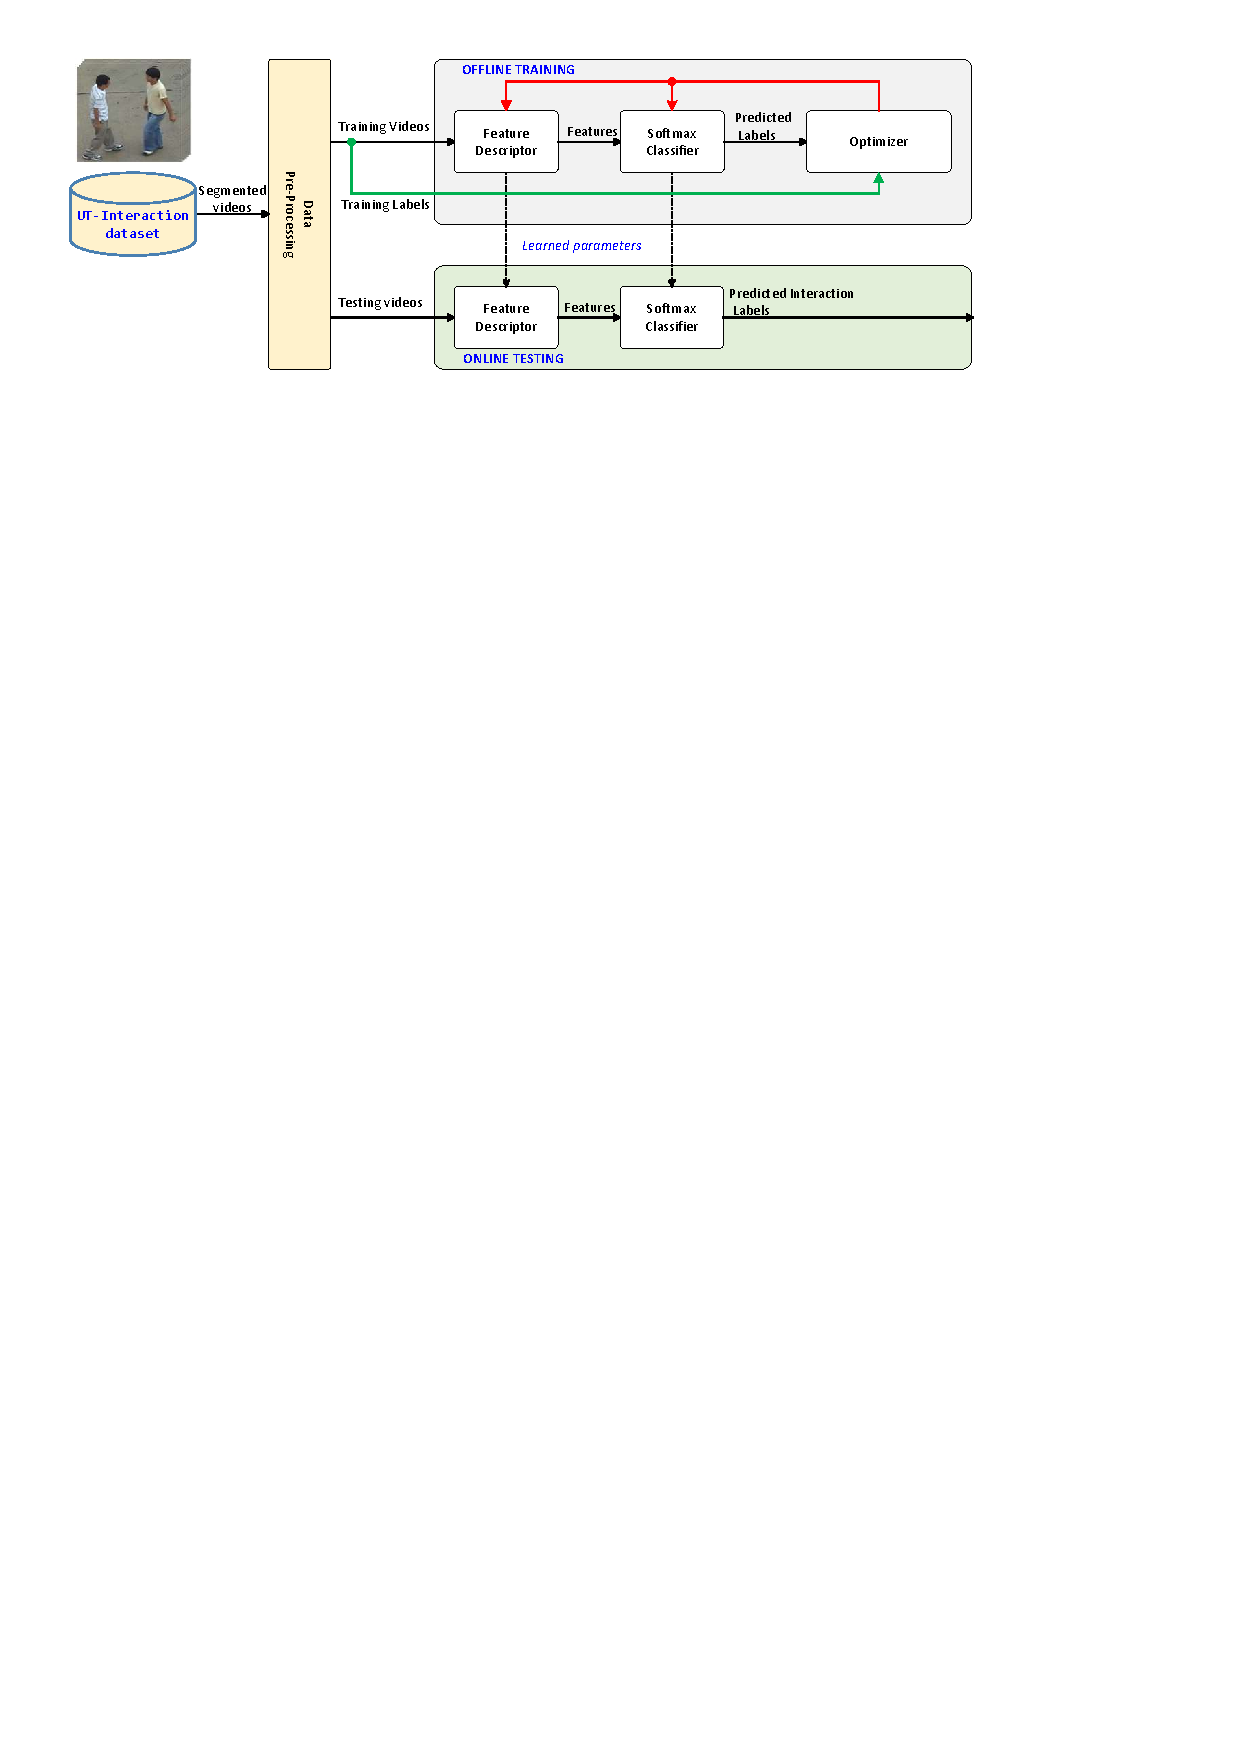
\includegraphics[trim=1cm 23cm 0cm 1cm]{fig01/dataflow_classifier.pdf}
	\caption{The overall data-flow of the interaction classification}
	\label{fig:df_classifier}
\end{figure}

\subsection{Data pre-processing}
The input videos of the global interaction feature descriptor contain two interacting people while the input videos of the atomic action feature descriptors contain only one of the two interacting people. So, the data pre-processing module need to generate different type of training and testing videos according to their corresponding feature descriptors. 
\par
The overall data-flow of data pre-processing module is illustrated in Figure \ref{fig:vpp}. The person segmentation module is designed to detect and track each person in the interaction videos and to segment each video into two videos which contain only one person in each video. There are three low-level data pre-processing modules, one for global interaction feature descriptor and the other two for the atomic action feature descriptors. These three low-level feature descriptors are synced to each other in order to ensure that they are processing the same video at the same time. The low-level data pre-processing module first splits the input videos into training set and testing set, then augments the training data by horizontal flipping and random chopping since the UT-Interaction dataset is a relative small scale interaction dataset for training a deep learning network, and finally resizes and clips the augmented videos into the video clips with proper size which can be accepted by the corresponding feature descriptors.  
\begin{figure}
	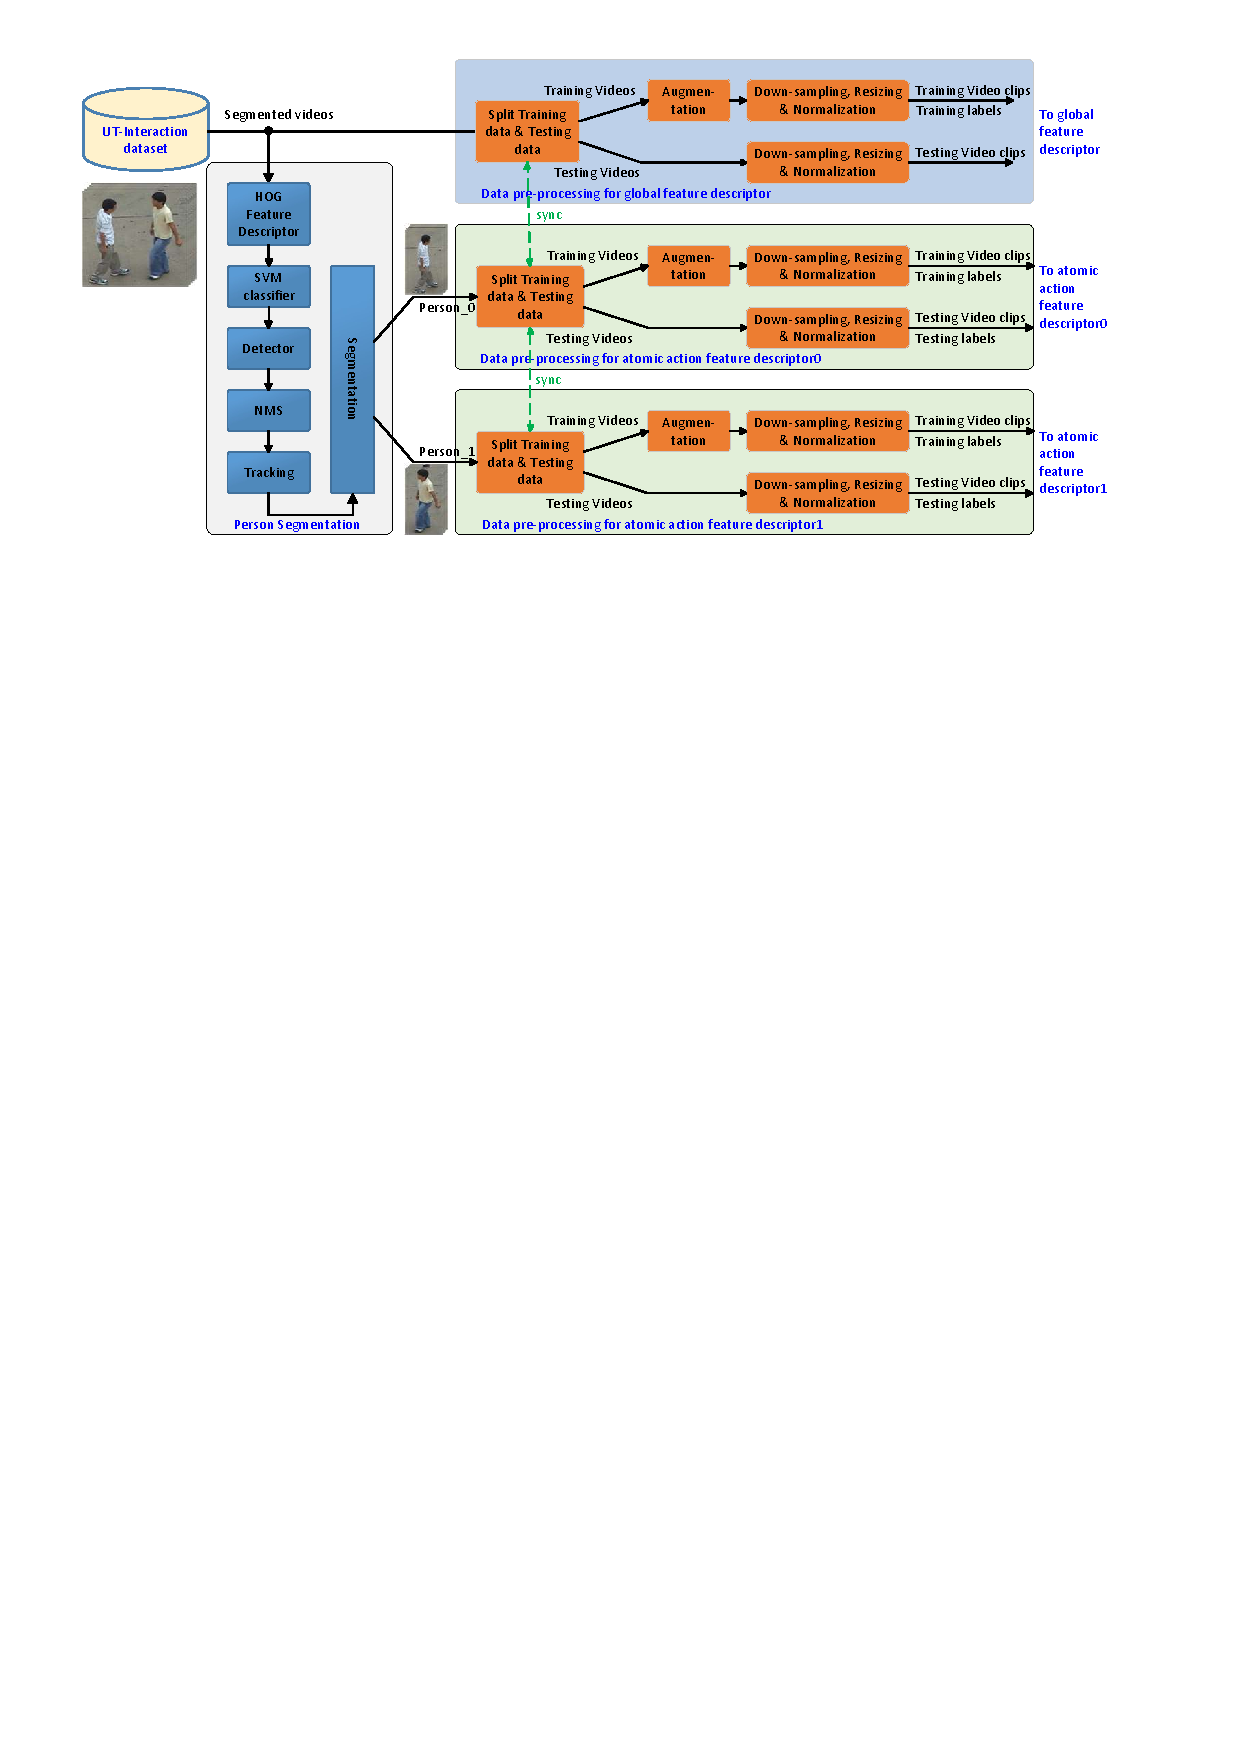
\includegraphics[trim=2cm 20.5cm 0cm 1cm]{fig01/vpp.pdf}
	\caption{The overall data-flow of the data pre-processing module}
	\label{fig:vpp}
\end{figure}

\subsubsection*{Person Segmentation}
\label{personDetection}
The tracking-by-detection methodology is employed in the person segmentation module. We first detect all people in each frame with a classical Histogram of Orientated Gradient (HOG) feature descriptor plus a linear support vector machine (SVM) classifier \cite{hog}. Then a Kalman filter is applied to track each person throughout a video. Since there are two and only two interacting people in the input videos, we get two-bounding boxes in each frame after tracking. And finally, we chop the video according to the bounding boxes and generate two segmented videos from each input video.

\paragraph*{The HOG feature descriptor}
The HOG feature descriptor is widely used to represent the appearance and shape of objects by calculating and collecting the gradients. The steps of generating HOG features include:
\begin{enumerate}
	\item Convert the input colourful image to gray scale.
	\item Calculate the gradients of each pixel. Specifically, the gradients for a pixel point at \((x,y)\) is calculated with following formulas:
	\begin{eqnarray}
		G_x(x,y) = H(x+1,y) - H(x-1,y) \\
		G_y(x,y) = H(x,y+1) - H(x,y-1) \\
		G(x,y) = \sqrt{G_x(x,y)^2 + G_y(x,y)^2)} \\
		\alpha(x,y) = tan^{-1}(\frac{G_y(x,y)}{G_x(x,y)})
	\end{eqnarray}
	Where \(G_x(x,y)\) and \(G_y(x,y)\) are the horizontal and vertical gradients respectively and \(H(x,y)\) is the pixel value of the point \((x,y)\). \(G(x,y)\) and \(\alpha(x,y)\) are the amplitude and orientation of the gradient of the pixel point \((x,y)\), respectively.
	
	\item Compute the histogram of gradients in the cell unit. A cell is usually composed of \(6 \times 6\) pixels and we use \(9\) bins to compute the histogram for these \(36\) pixels. The value of orientation determines which bin need to add and the value of amplitude determines the weight of adding.
	
	\item Normalize the histogram in a bigger block unit. A block is usually composed of \(3 \times 3 \)  neighbor cells by doing which we can further eliminate the effects of different lighting and contrast of the raw images.  There are \(3 \times 3 \times 9 \) features for each block.
	
	\item Slide the block horizontally and vertically with stride \(j=1\ cell\), we get many blocks and their features \(x_i\). All those features are combined together as \(\{x_0, x_1,...,x_n\}\) as the finally HOG features of an image.
\end{enumerate}

\paragraph*{The linear SVM classifier}
In our project, we use a linear SVM to determine whether the input image is a person or not according to the input features extracted by the HOG feature descriptor. The object of training such a liner classifier is to find a hyper-plane which is defined as:
\begin{equation}
	w^Tx + b = 0
\end{equation}
Where \(x\) is the input features, \(w\) and \(b\) are the weights and biases respectively. We get the optimal values of \(w\) and \(b\) by training the classifier on the INRIA dataset \cite{inria_person}. Then we use \(h_{w,b}(x) = g(w^Tx+b)\) to predict whether the input is a person or not. The input is predict as a person if \(h_{w,b}(x) \geq 0 \), and vice versa.

\paragraph*{Person detection} 
A sliding window is used to detect the locations of the interacting people in each frame. A size variable window slides over the whole image with stride \((4,4)\), and the pixels in the sliding window will be converted to HOG features and predicted by the SVM classifier. For the purpose of scale invariant, we apply the detection in multi-scale image pyramid. The multi-scale image pyramid is composed of the images with different scales with the below formula. 
\begin{equation}
	img\_cols_{i+1}, img\_rows_{i+1} = \frac{img\_cols_i}{scale}, \frac{img\_rows_i}{scale}
\end{equation}
Where \(img\_cols_i\) and \(img\_rows_i\) are the width and height, respectively, of the image in the \(ith\) layer of the image pyramid, and \(scale = 1.03\) controls the shape and the number of layers of the image pyramid. 
The location, window size as well as the confidence will be recorded if it is predicted as a person. Since there are many overlapping windows after the whole detection process, we use non-maximum-suppression (NMS) to eliminate the overlapping windows and find out those windows with maximum confidence. The overlap threshold is set to 0.65 in the project. 

\paragraph*{Tracking of people} 
The detection of one or two person may loss in some frames. So, we employ the second order Kalman filter to track the location of each person throughout the whole videos. There are exactly two interacting people to track in our project, so, we have two independent Kalman filters. Instead of tracking a whole bounding box, we use the Kalman filter to track the left-top point location of each bounding box, and reconstruct bounding boxes with the filtered left-top point locations plus the average width and height of all the bounding boxes in the video.  
\par 
Another special point in our project is that the relative left-right position between the two interacting people will keep unchanged. That is, if the person A first present at the left side of the two interacting people, then he will always be at the left side throughout the whole video.  So, we do not need to specially design a algorithm to match the people when tracking but just simply assign the left bounding box to person A and the right one to person B.  The detail design of the Kalman filter for a single person is introduce as below.
\par
The system state of each person includes position, velocity, and acceleration. We do not use acceleration in our Kalman filter since it varies very much when people are interacting. We notate the position at time \(t\) as \(p(t) = (x(t),y(t))\) and the system state at time \(t\) is \(x(t) = [p(t), v(t)]\). Then we implement the Kalman filter with following steps:
\begin{enumerate}
	\item Initialize the Kalman filter.
	\begin{eqnarray*}
		t \leftarrow 0 \\
		Q(0) = I_4 * 10^{-6} \\
		R(0) = I_4 * 10^{0}
	\end{eqnarray*}
	Where \(I_4\) is a \(4 \times 4\) identity matrix. \(Q(0)\) and \(R(0)\) are the initial value of the noise covariance matrices for estimation and measurement, respectively. 
	\item Estimate the system states at time \(t\) according to the optimal value of the system state at time \(t-1\).
	\begin{equation}
		\left[
		\begin{matrix}
		p(t|t-1) \\
		v(t|t-1)
		\end{matrix}
		\right] =
		\begin{bmatrix}
		I_2&I_2\\
		O_2&I_2 \\
		\end{bmatrix}
		\begin{bmatrix}
		p(t-1|t-1) \\
		v(t-1|t-1)
		\end{bmatrix}
		+ w(t)
	\end{equation} 
	Where \(I_2\) and \(O_2\) are \(2 \times 2\) identity and null matrices, respectively. \(w(t)\) represents the uncertainty of the estimation, and is assumed to be a random variable with a zero mean and its covariance matrix \(Q(t) = E[w(t)w^T(t)]\).
	
	\item Update the covariance matrix for the estimation of the system states at time \(t\) according to the covariance matrix of the system sate at time \(t-1\). 
	\begin{equation}
		P(t|t-1) = \begin{bmatrix}
		I_2&I_2 \\
		O_2&I_2
		\end{bmatrix} P(t-1) + Q(t)
	\end{equation}
	Where \(P(t|t-1)\) is the covariance matrix of the estimation at time \(t\), and \(P(t-1)\) is the covariance matrix of the optimal system states at time \(t-1\).
	
	\item Measure the system states at time \(t\). 
	\begin{equation}
	 \begin{bmatrix}
	 \bar p(t) \\
	 \bar v(t)
	 \end{bmatrix}
	 = 
	 \begin{bmatrix}
	I_2&O_2
	\end{bmatrix}
	\begin{bmatrix}
	\bar p(t) \\
	\bar p(t) - p(t-1|t-1)
	\end{bmatrix}
	+m(t)
	\end{equation}
	Where \(\bar p(t)\), \(\bar v(t)\) are the measured system states at time \(t\). If the detection of the person is missing in some frames, we use the measured values at the time \(t-1\) as the measure value at time \(t\).    \(m(t)\) is the uncertainty of the measurement, and is assumed to be a random variable with a zero mean and its covariance matrix \(R(t) = E[m(t)m^T(t)]\).
	
	\item Update the Kalman gain at time \(t\) according to the covariance matrix of the estimation of the system states at time \(t\).
	\begin{eqnarray}
	Kg(t) = \frac{P(t|t-1) H^T}{HP(t|t-1) H^T + R(t)} \\
	H = 
	\begin{bmatrix}
	I_2&O_2 \\
	O_2&I_2
	\end{bmatrix}
	\end{eqnarray}
	Where \(Kg(t)\) is the Kalman gain at time \(t\).
	
	\item Calculate the optimal system states according to the estimation, measurement and the value of Kalman gain.
	 	
	\begin{equation}
	\begin{bmatrix}
	p(t|t) \\
	v(t|t)
	\end{bmatrix}
     =
     \begin{bmatrix}
     p(t|t-1) \\
     v(t|t-1)
     \end{bmatrix} + Kg(t) \left(
     \begin{bmatrix}
     \bar p(t) \\
     \bar v(t)
     \end{bmatrix} - 
     \begin{bmatrix}
     I_2&O_2 \\
     O_2&I_2
     \end{bmatrix}
      \begin{bmatrix}
     p(t|t-1) \\
     v(t|t-1)
     \end{bmatrix} \right)
	\end{equation}
	
	\item Update the covariance matrix for the optimal system states at time \(t\) according to the Kalman gain and covariance matrix of the estimated system sate at time \(t\). 
	\begin{equation}
	P(t|t) = \left(1-Kg(t)\begin{bmatrix}
	I_2&O_2 \\
	O_2&I_2
	\end{bmatrix}\right)P(t|t-1)
	\end{equation}
	
	\item Repeat above steps from 2 to 7 at time \(t+1\).
\end{enumerate}

We generate a bounding box for each person in each frame after tracking, and the width and height of all bounding boxes are the same because we replace the width and height of each bounding box with the average value of the width and heigh of all bounding boxes in a video based on a reasonable assumption that every people appeared in the video have similar width and height. Finally, we crop the interaction video according the bounding boxes and generate two segmented videos which contain one person in each. See the inputs and outputs of the Person Segmentation module in the Figure \ref{fig:vpp}.

\subsubsection*{Data pre-processing}
\label{pre_processing}
The functions of data pre-processing include: splitting of training and testing data, augmentation of training data and converting the training and testing videos to proper size which can be accepted by the corresponding feature descriptors.  The general steps of data pre-processing are:
\begin{enumerate}
	\item The splitting of training and testing data. Since UT-Interaction is a  relative small scale interaction video dataset, we use 10-fold leave-one-out cross validation to evaluate the performance. There are 10 sequences in each set, and 6 videos in each sequence. So, we leave one sequence for testing and other nine sequences for training in each run. See \ref{ut-interaction} for detail.
	\label{augmentation}
	\item Augmentation of training data.  After the splitting of training and testing videos, we get 56 videos for training and 6 videos for testing in each run. But, 56 videos is not sufficient to train our deep learning network. So, we employ two methods, horizontal flipping and random chopping, to augment the training videos. Horizontal Flipping is used to generate a new video by horizontally flipping each frame from the original video which is illustrated in Figure \ref{fig:flip_4}. We further enlarge the scale of the training set \(n\) times by N-time random cropping. In the random cropping module, we chop the video by a window with fixed size and random position of left-top point in a reasonable range. Specifically, in our project, we first resize each training video to \(l \times 128 \times 144\), where \(l\) is the number of frames for each video, then random chop each video with size \(l \times 112 \times 128\). An example of the random cropping is illustrated in Figure \ref{fig:cropping_4}.
	\label{down-sampling}
	\item Down sampling. The number of frames of each individual interaction video is usually in the range from 60 to 150 frames, but our feature descriptor can only accept the video clips with only 16 frames due to the limitation of GPU memory and computation time. If we directly chop each video into 16-frame video clips, then there will be only very limited temporal information contained in each video clip. So, we first down-sample the video with \(N\) frames stride to make each video clip contains more temporal information. Besides the fixed stride temporal down-sampling, we have an additional temporal down-sampling mode, that is, we  sample exactly 16 frames from each input video with equal distances if the number of frames of the input video is larger than 16 by setting \(N=0\).  
	
	\item Resizing. The number of frames for each video may be still larger than 16 after down sampling of frames, then we chop them to many 16-frame video clips with 8 frames over-lapping.
	\label{normalization}
	\item Normalization. Since our training data are videos, the most common method of normalization videos is to subtract the mean value of all pixels which is calculated across all training videos. To further eliminate the affect of different lighting, we divide the value of every pixel by the standard deviation with following formulas: 
	\begin{eqnarray}
		\mu = \frac{\sum_{m,l,h,w,c}p_{m,l,h,w,c}}{N} \\
		std = \sqrt{\frac{\sum_{m,l,h,w,c}(p_{m,l,h,w,c}-\mu)^2}{N}} \\
		p_{Norm} = \frac{p_{m,l,h,w,c} - \mu}{std}
	\end{eqnarray} 
	Where \(m\),\(l\),\(w\),\(h\),\(c\) are the number of video clips, the number of frames per video clip, the width, height and the number of channels per frame respectively.  \(p_{m,l,h,w,c}\) is the pixel value, \(\mu\) and \(std\) are the mean value and standard deviation of pixels over all training videos. And the \(p_{Norm}\) is a generated pixel value after normalization. 
\end{enumerate} 

\begin{figure}
	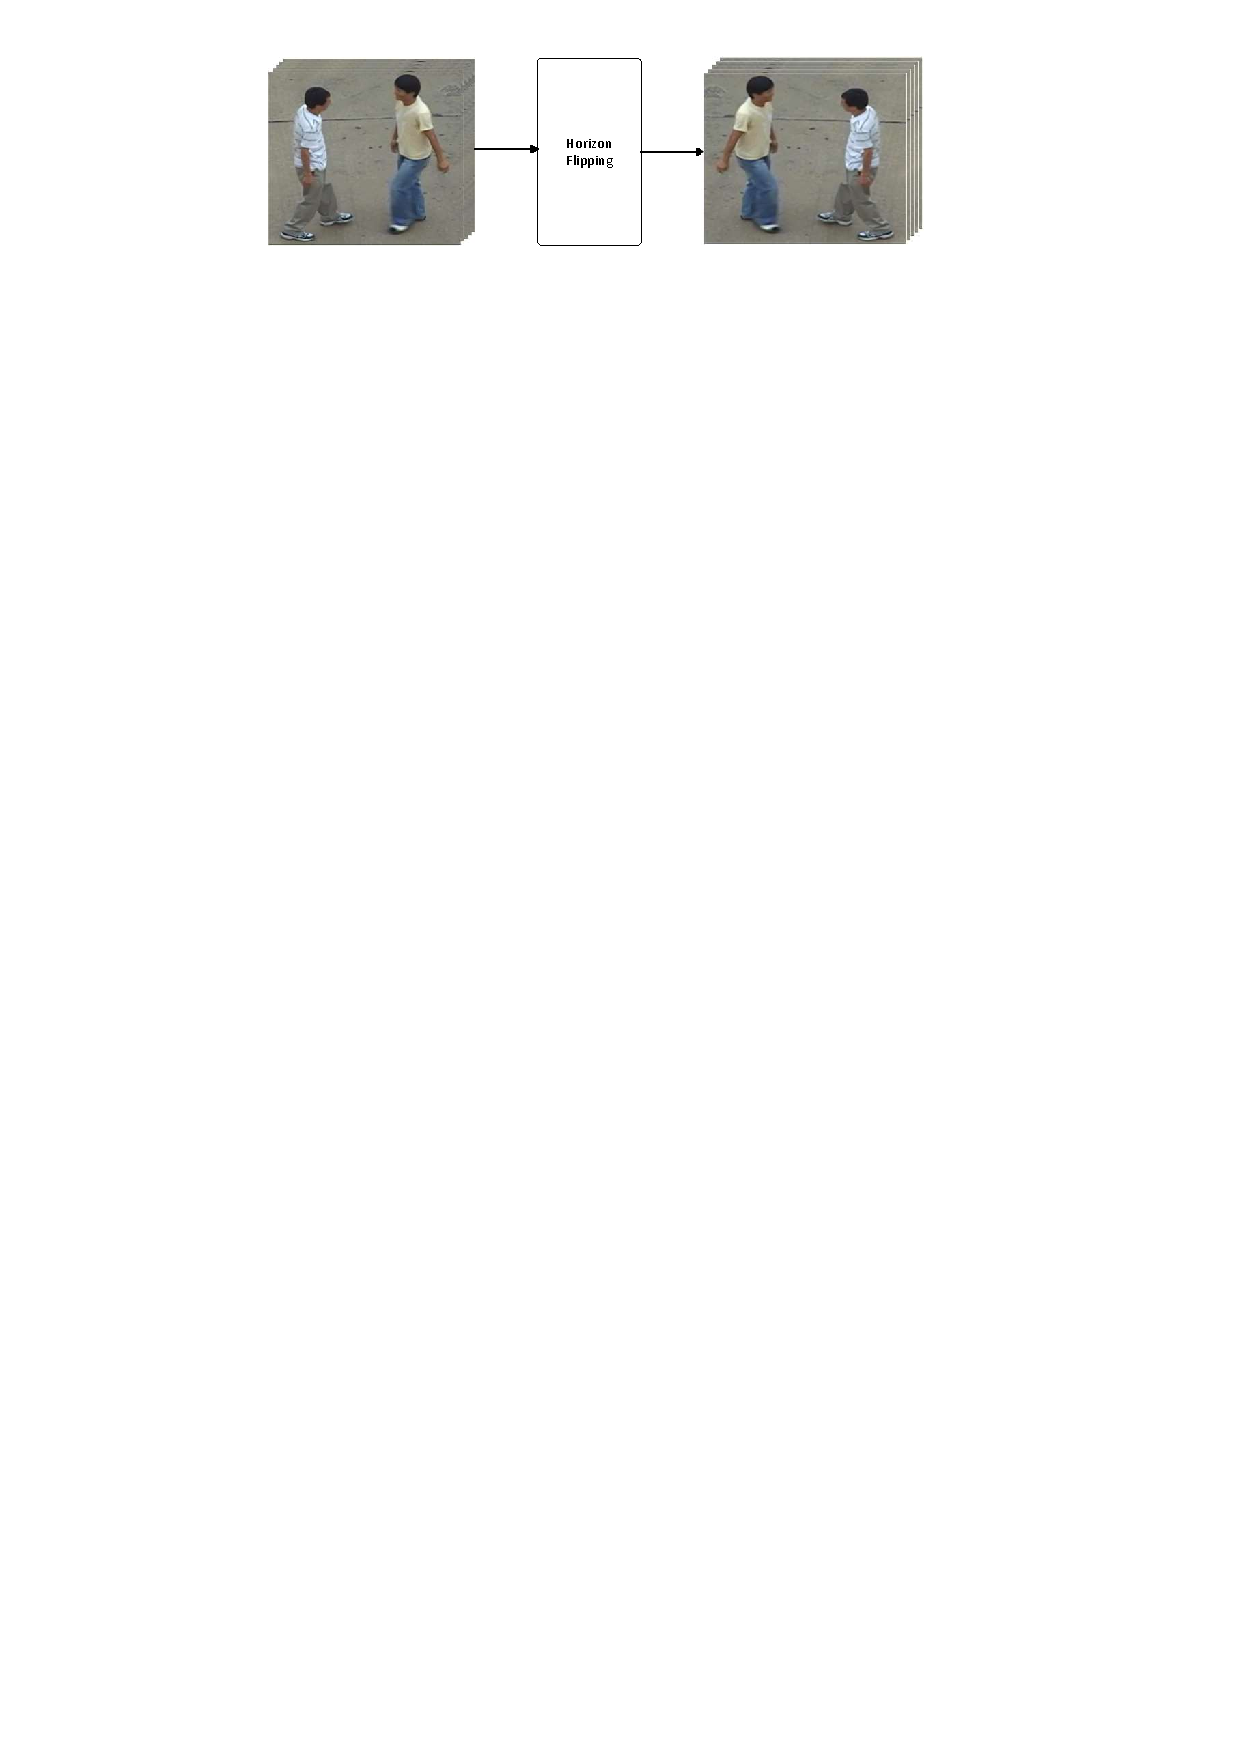
\includegraphics[trim=2cm 25.5cm 0cm 1cm]{fig01/flip.pdf}
	\caption{Horizontal flipping of a video}
	\label{fig:flip_4}
\end{figure} 
\begin{figure}
	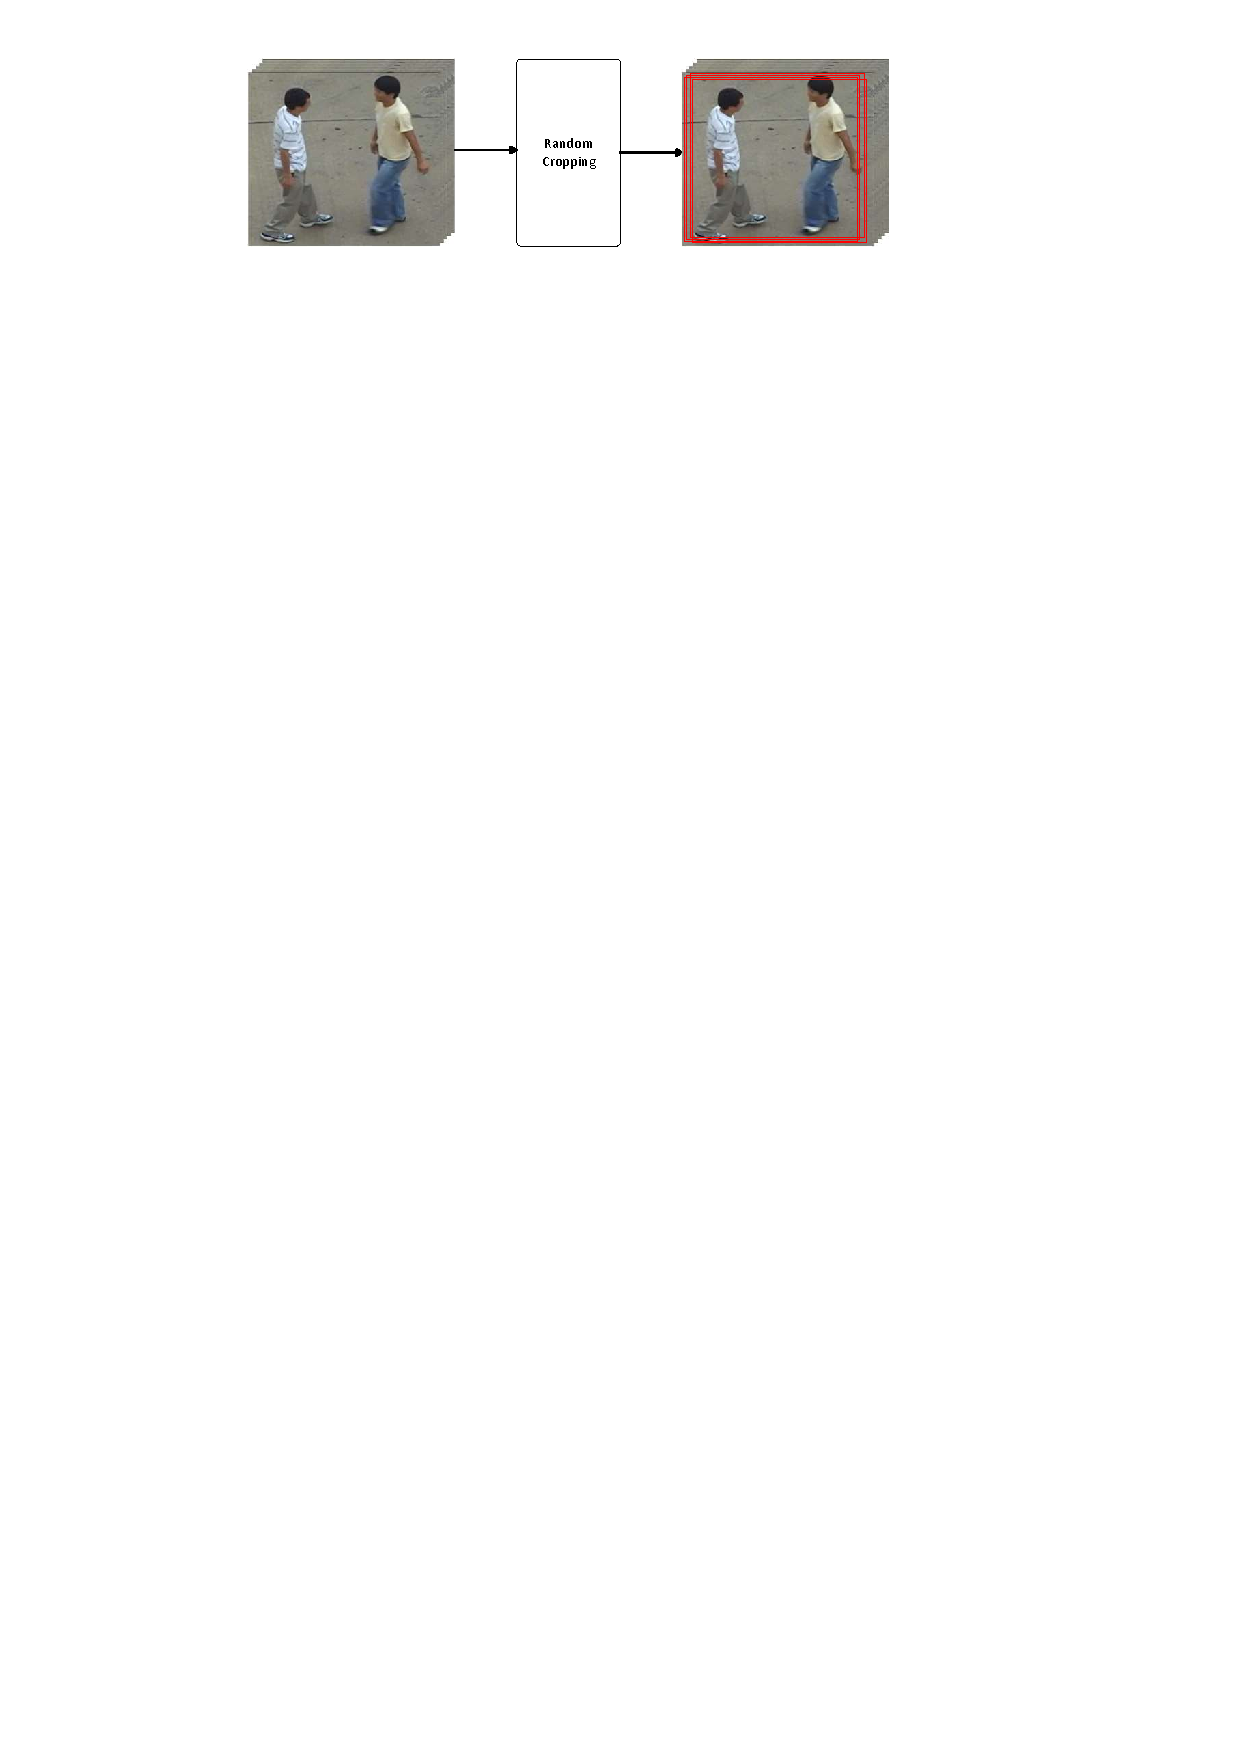
\includegraphics[trim=2cm 25.5cm 0cm 1cm]{fig01/cropping.pdf}
	\caption{Random cropping a video}
	\label{fig:cropping_4}
\end{figure}  
   
\subsection{Feature descriptor}
To fully represent the features of the input interaction videos, we employ a hierarchical feature descriptor which contains one global interaction feature descriptor and two atomic action feature descriptors. All the three feature descriptors are based on a same structure 3D ConvNet but with different size of input videos and network parameters. The input video's size for global interaction feature descriptor is \(n \times 16 \times 112 \times 128 \times 3\) while that for the atomic action feature descriptors is \(n \times 16 \times 112 \times 80 \times 3\), where \(n\) is the number of video clips, \(l = 16\) is the number of frames of each video clip, \(112 \times 128 \times 3\) and \(112 \times 80 \times 3\) are the frame sizes for the global interaction feature descriptor and the atomic action feature descriptors respectively. The structure of feature descriptor is illustrated in Figure \ref{fig:feature_descriptor}.  
\par
\label{3dconv_layers}
The Architecture of the 3D ConvNet is illustrated in Figure \ref{fig:3DConvNet_4}. The 3D ConvNet feature descriptor contains 4 3D convolutional and pooling layers and 2 fully connected layers.  
\begin{figure}
	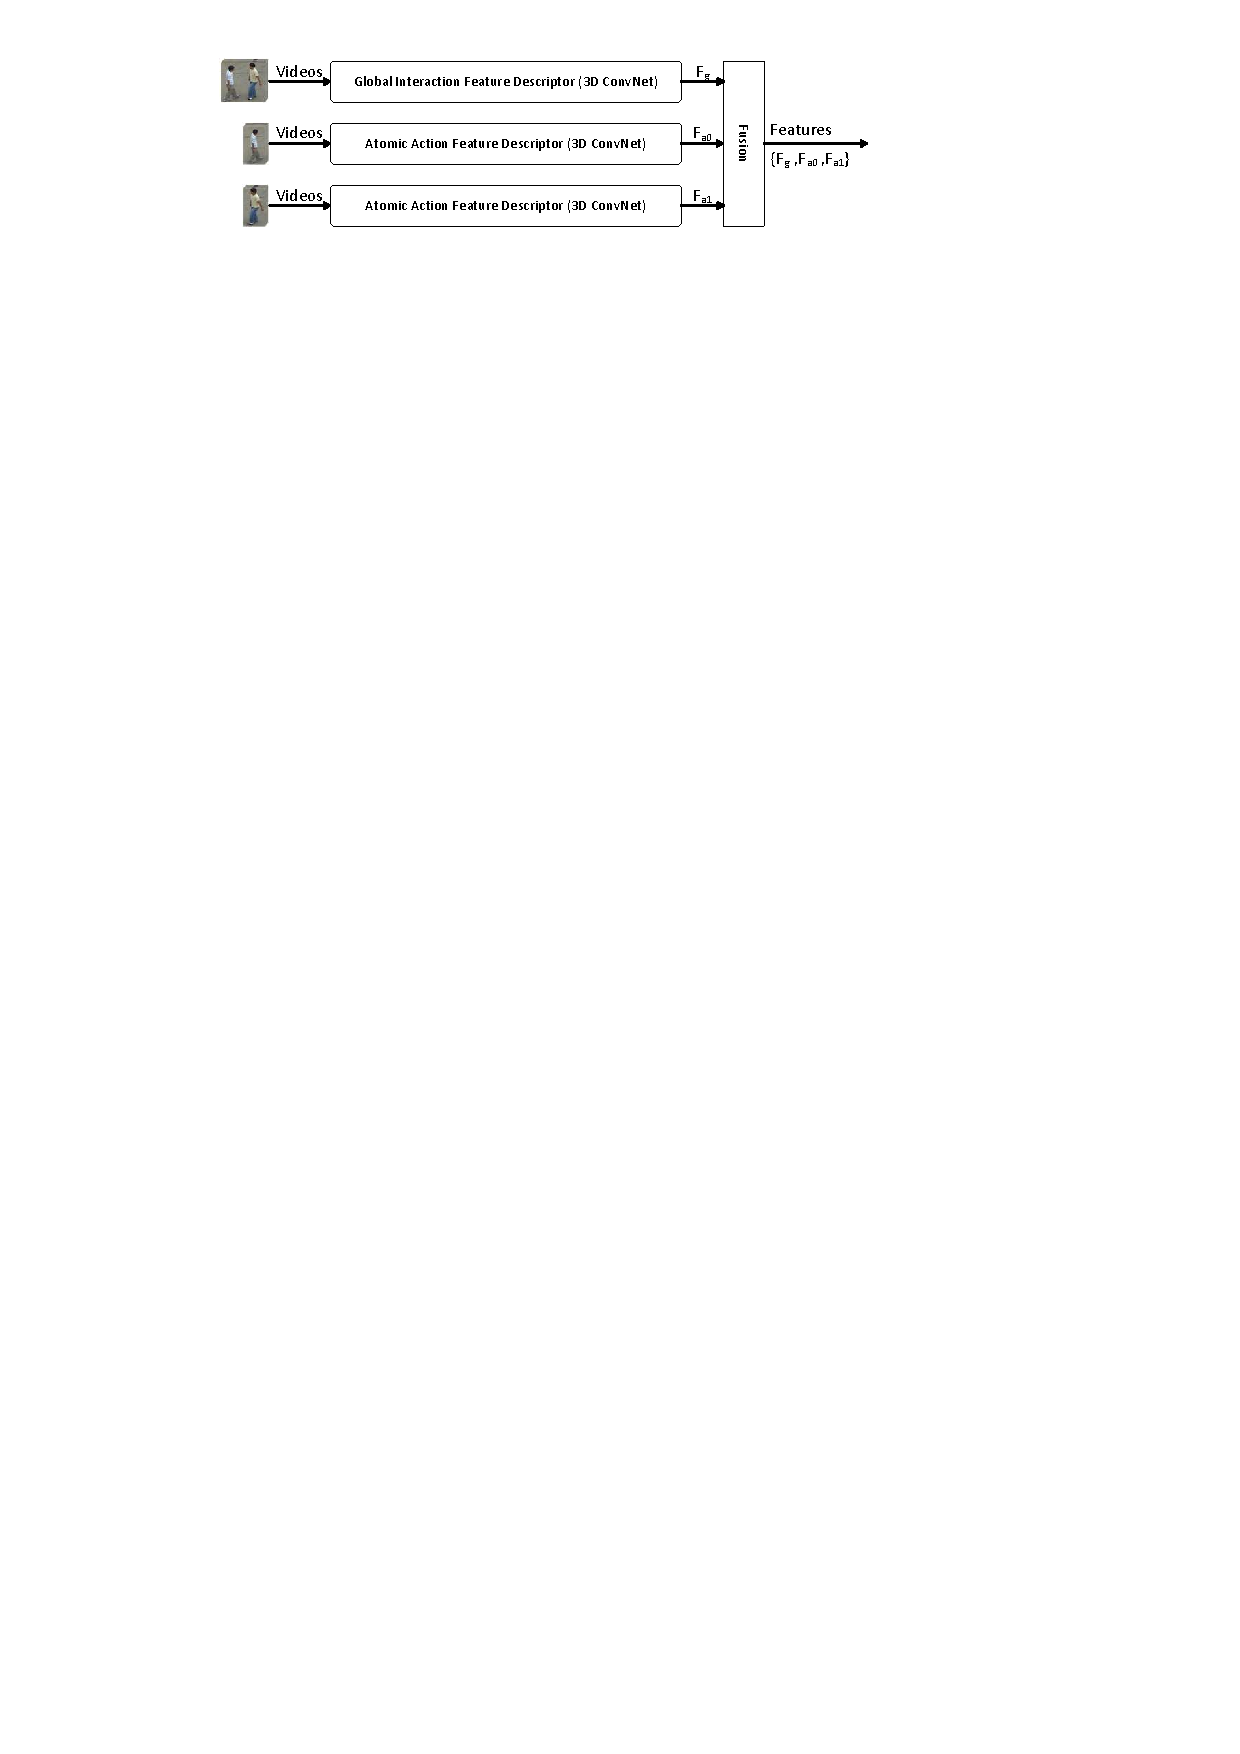
\includegraphics[trim=2cm 25.5cm 0cm 1cm]{fig01/feature_descriptor.pdf}
	\caption{The structure of the feature descriptor}
	\label{fig:feature_descriptor}
\end{figure} 
\begin{figure}
	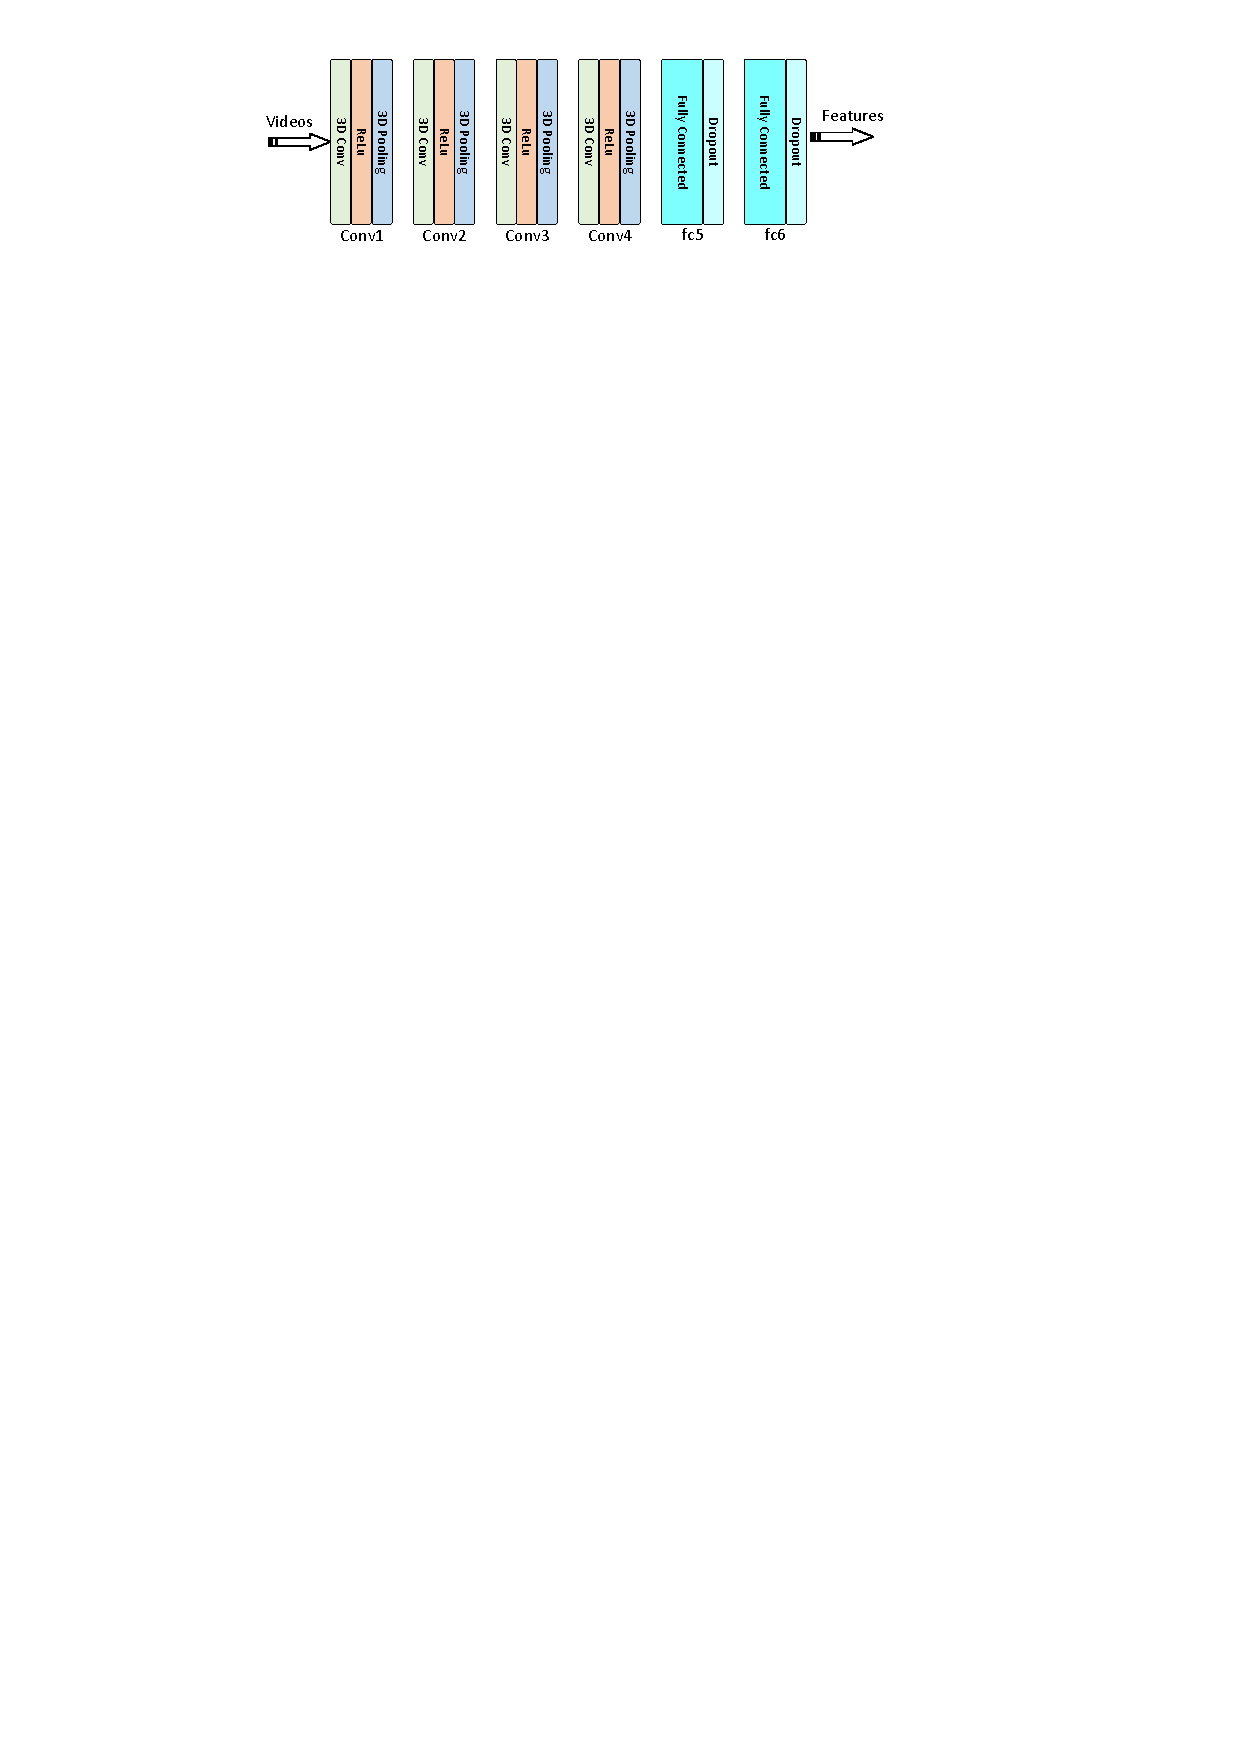
\includegraphics[trim=2cm 25.5cm 0cm 1cm]{fig01/3DConvNet.pdf}
	\caption{The architecture of the 3D ConvNet}
	\label{fig:3DConvNet_4}
\end{figure}

\subsubsection*{The 3D convolutional and pooling layer}
Each 3D convolutional and pooling layer contains three main operations: 3D convolution, Rectified Linear Unit (ReLU) and pooling as shown in Figure \ref{fig:3DConvNet_4}. We also introduce two Batch Normalization \cite{bn} layers after the first two pooling layers.   
\paragraph*{3D convolution:}
\label{3dconv_filters}
Different from a 2D convolutional layer which only applies convolution spatially, the 3D  convolutional layer applies convolution spatially and temporally, thus, it can extracts both spatial and temporal features. In our project, the input of the 3D convolutional layer is a 5D volume with size \([n,l,h,w,c]\) and the size of the 3D filter is \([d,k,k,c]\). The 3D filter convolves a 3D volume which has the same shape with it in the input video. Then the 3D volume slides spatially and temporal across over the whole input video to generate a new output 3D volume which has the same shape as the input video (if boundary padding is applied) except all input channels are summed. The 3D convolution can be described as the following formula: 
\begin{equation}
	Output_{n,i,j,k} = \sum_c \sum_{di,dj,dk}^{h,w,l} In_{n, i + di, j + dj, k + dk} * Filter_{di,dj,dk}
\end{equation}
Where \(n\) is the number of video clips, \(l\) is the number of frames per video clip, \(h,w,c\) are the height, width and number of channels per frame respectively. \(In_{n,l,h,w,c}\) is the pixel value at the specified position. \(i,j,k\) are the offsets of the sliding window with strides 1. \(Filter[di,dj,dk]\) is the value of the filter at point \([di,dj,dk]\). 
\par 
There are \(nof\_conv\) filters in each convolutional layer. Each filter convolves the input volume separately, and all the outputs of the convolutional results are concatenated together as the final output of a convolutional layer. For example, \([16,16,112,128,3]\) is the shape of an input volume which has 16 video clips, 16 frames with size \([112,128,3]\) per video clips , \([3,3,3,3,32]\) is the shape of the filters which have 32 filters with size \([3,3,3,3]\). The last \(3\) is the number of channels which must be as same as the number of channels of the input volume. 

\paragraph*{ReLU:}
An additional operation called Rectified Linear Unit (ReLU) is employed after every convolution operation. The purpose of ReLU is to introduce non-linearity in our 3D ConvNet. The ReLU is an pixel wise operation and replaces all negative pixel values of the output of convolutional layer by zero which is defined in Figure \ref{fig:relu} and following formula:
\begin{equation}
Output = Max(0,Input)
\end{equation} 

\begin{figure}
	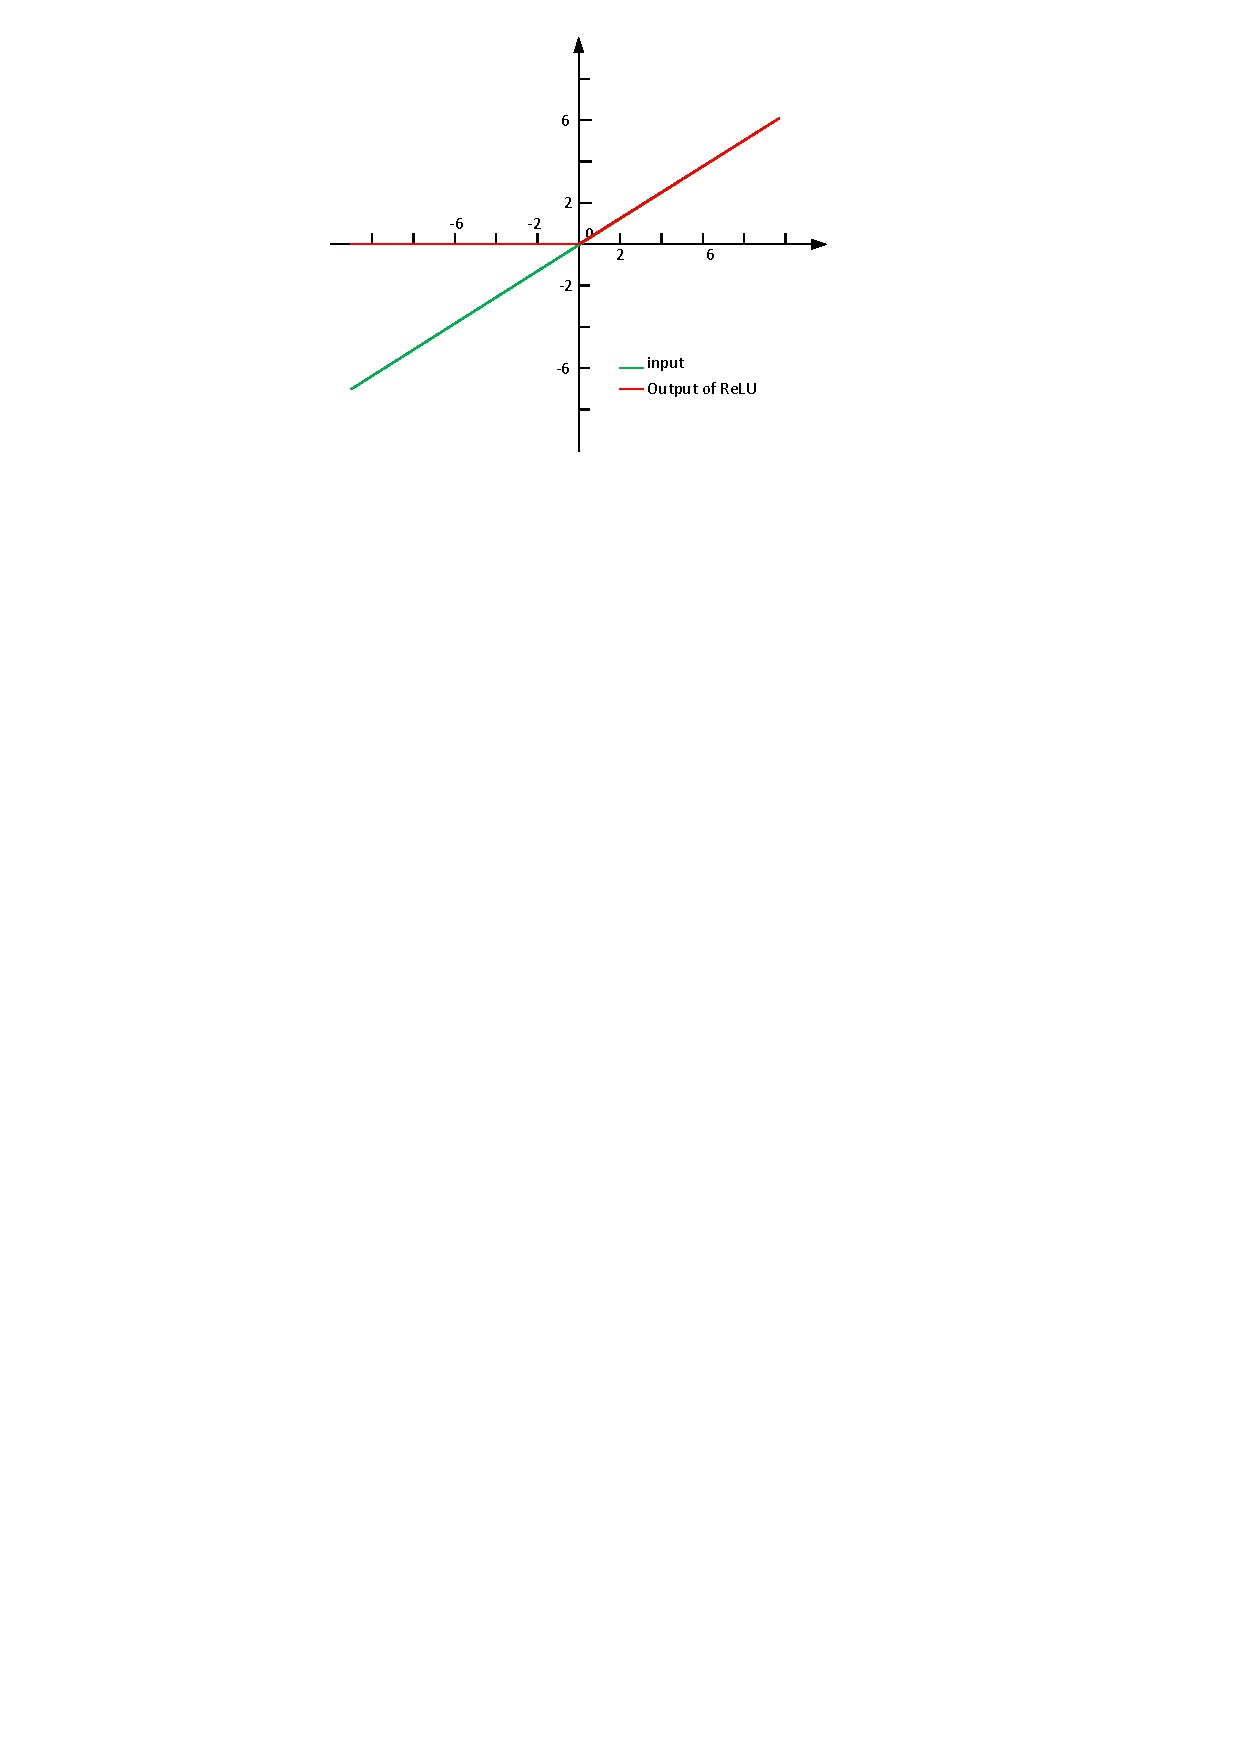
\includegraphics[trim=2cm 22cm 0cm 1cm]{fig01/relu.pdf}
	\caption{The illustration of the ReLU operation}
	\label{fig:relu}
\end{figure}

\paragraph*{Batch Normalization}
\label{bn}
Batch normalization alleviates a lot of headaches with properly initializing neural networks by explicitly forcing the activations throughout a network to take on a unit Gaussian distribution at the beginning of the training. Batch normalization is performed to each neuron. The forward propagation steps are shown as below:
\begin{enumerate}
	\item Calculate the mean value and variance over the input mini-batch.
	\begin{eqnarray}
		\mu_B = \frac{1}{m} \sum_{i=1}^m x_i \\
		\sigma_B^2 = \frac{1}{m} \sum_{i=1}^m (x_i - \mu_B)^2
	\end{eqnarray}
	Where \(\mu_B\) and \(\sigma_B^2\) are the mean and variance of the input mini-batch, respectively.
	
	\item Normalize the input mini-batch.
	\begin{equation}
		\hat{x_i} = \frac{x_i - \mu_B}{\sqrt{\sigma_B^2 + \epsilon}}
	\end{equation}
	
	\item Scale and shift the normalization results to reconstruct the data.
	\begin{equation}
		y_i = \gamma \hat{x_i} + \beta
	\end{equation}
\end{enumerate}
In the training phase, \(\gamma\) and \(\beta\) are updated by the optimizer, and in the testing phase, the mean values of \(\gamma\) and \(\beta\) are used.


\paragraph*{Max pooling:}
\label{pooling}
According to the previous researches \cite{Tran2015} \cite{3dcnn_1}, max pooling performs better in the 3D ConvNet than other methods of pooling, so, we also employ 3D max pooling in our 3D ConvNet. The purpose of operating max pooling is to reduce the dimensionality of each feature map but retains the most important information. In our project, we define a spatial and temporal neighbourhood (a \(2 \times 2 \times 2\) window) and take the largest element in that window. 

\subsubsection*{Fully connected layer}
\label{fc}
A fully connected layer is a traditional multi-layer perception where every neurons in the previous layer is connected to every neurons in the next layer. The outputs from the convolutional and pooling layers represent high-level features of the input video clips, while the fully connected layers are designed to learn some non-linear combinations of the output feature maps of the convolutional layers.
\par
\label{dropout}
To avoid overfitting to the training set, a dropout layer \cite{dropout} is added after each fully connected layer. While training, dropout is implemented by only keeping a neuron active with some probability \(p\), or setting it to zero otherwise. 

\subsubsection*{Fusion of features}
As mentioned at the beginning of this section, we have three sub feature descriptors in our hierarchical feature descriptor. The output features of these three feature descriptors are notated as \(F_g\) (features extracted by the global interaction feature descriptor ), and \(F_{a0}\),\(F_{a1}\) (features extracted by the two atomic action feature descriptors).  We concatenate the three sets of features as the final output features of our hierarchical feature descriptor, the final output features are notated as below:
\begin{equation}
 	Features = \{F_{g}, F_{a0}, F_{a1}\}
\end{equation}  

\subsection{Softmax classifier}
The output of our hierarchical feature descriptor is a vector with \(4096 \times 3\) dimensions. And we have 6 interaction classes for classification task and 7 interaction classes for detection task (one more class than classification is used to label the class which not belongs to anyone of the 6 interaction classes). As shown in Figure \ref{fig:softmax} we first transform the high dimension features to the scores for each classes: 
\begin{equation}
	h_{w,b}(X) = w^Tx + b
\end{equation}
Where \(w\),\(b\) are the weights and biases, respectively, and \(X\) is the input features. For example, the dimensionality of the input features is \(n \times 12288\) and we have 6 output classes, then the dimensionality of the weights should be \(12288 \times 6\) and the dimensionality of biases should be \(6\). 
\par 
We then apply softmax regression to convert the score of each class to probability distribution with the following formula:
\begin{equation}
	\left[
	\begin{matrix}
		p(y=1|x;w,b) \\
		p(y=2|x;w,b) \\
		p(y=3|x;w,b) \\
		. \\
		. \\
		. \\
		p(y=6|x;w,b)
	\end{matrix}
	\right] = \frac{1}{\sum_{j=1}^6 e^{h_{w_j,b_j}(X)}} \left[
	\begin{matrix}
		h_{w_1,b_1}(X) \\
		h_{w_2,b_2}(X) \\
		h_{w_3,b_3}(X) \\
		.\\
		.\\
		.\\
		h_{w_6,b_6}(X) \\		
	\end{matrix}
	\right]
\end{equation} 
The set the label which gets the maximum probability value as the predicted label for the input feature. 
\begin{figure}
	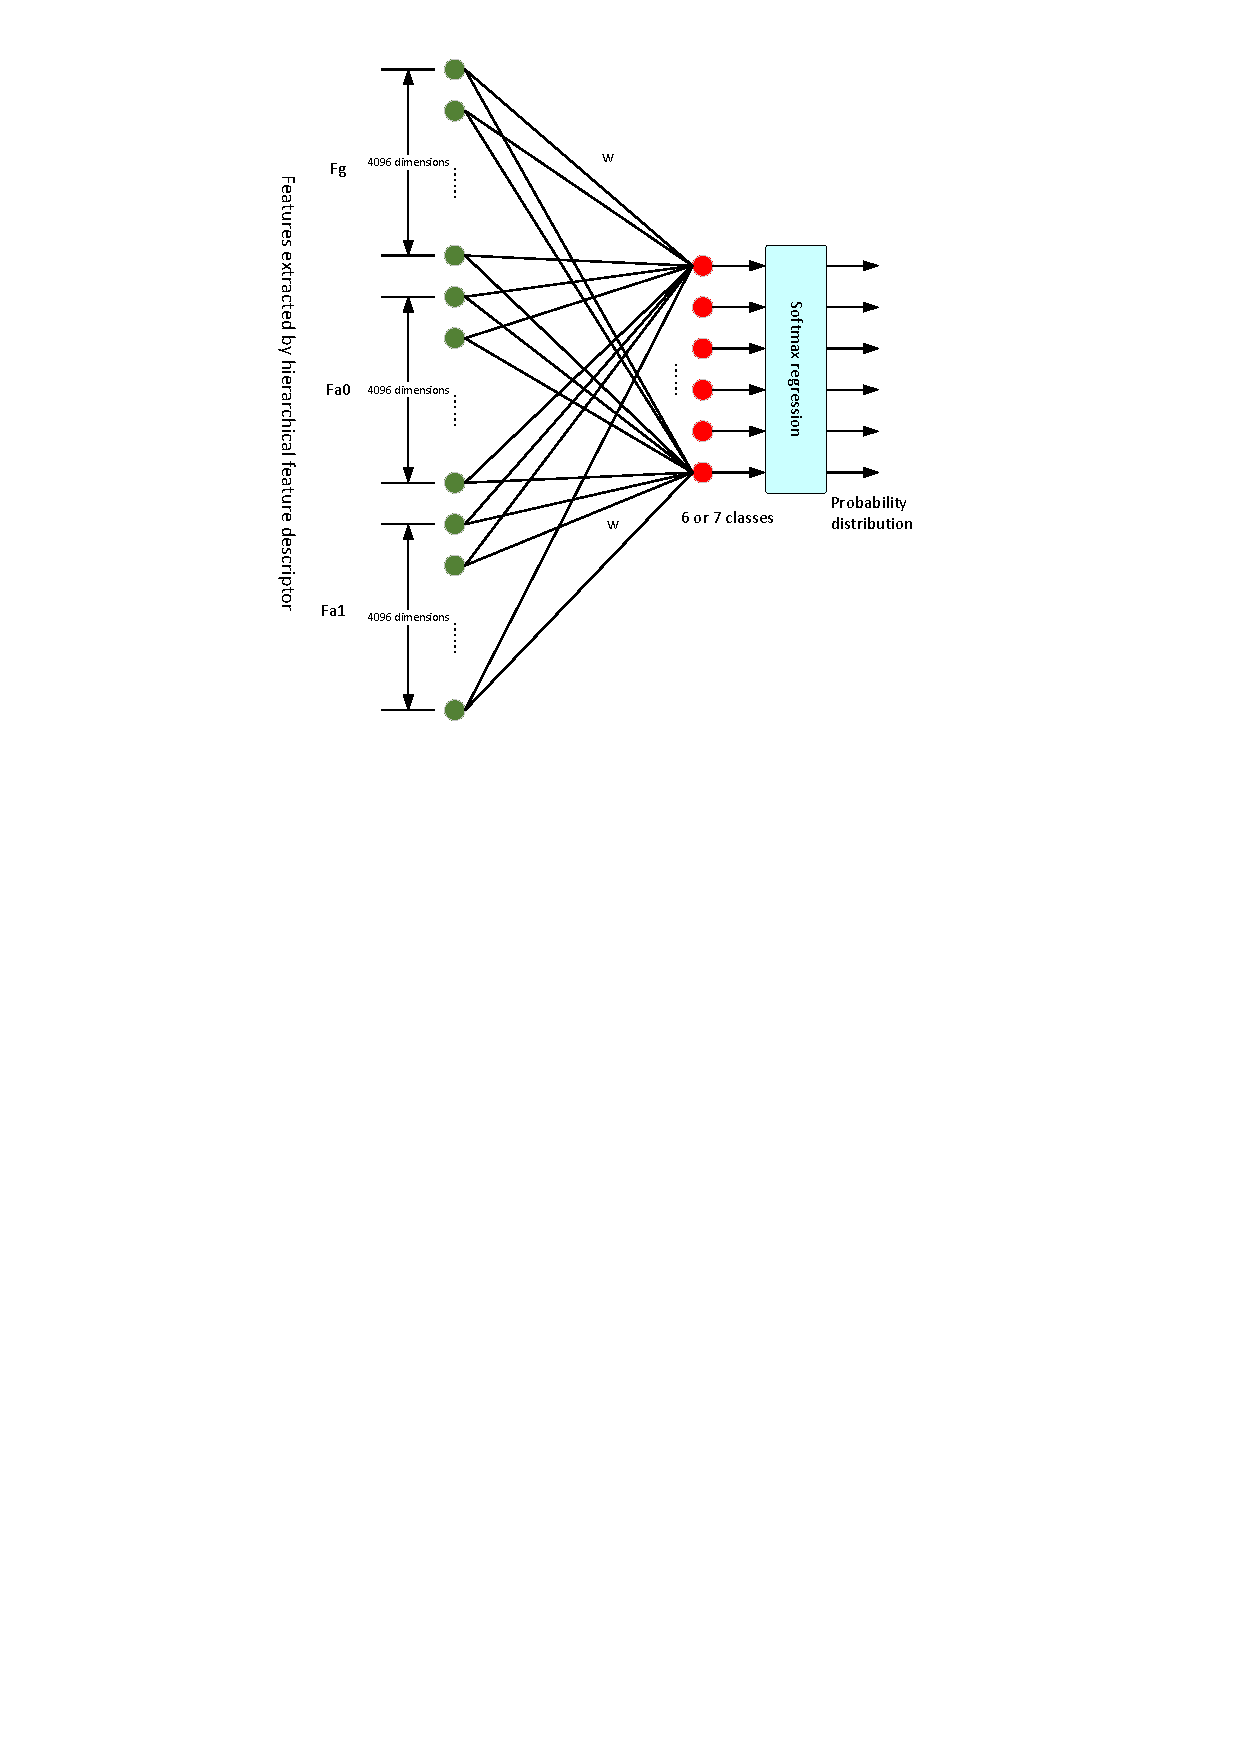
\includegraphics[trim=2cm 17cm 0cm 1cm]{fig01/softmax.pdf}
	\caption{The softmax classifier}
	\label{fig:softmax}
\end{figure}

\subsection{Optimizer}
The processes of optimization in our project are composed of initialization of the parameters, optimizing of the parameters  with the ADAM optimizer, dynamic adjustment of the learning rate. 
\subsubsection*{Initialization of the parameters}
\label{Initialization}
The network parameters, including weights and biases, are initialized before the optimizing process. We expect that weights to be small random numbers close to \(0\). So, we initialize all weights with a normal distribution with zero mean. And the value of biases are initialized to a constant value 0.  
\subsubsection*{Optimizing of the parameters}
\label{optimizer}
The objective of the optimizer is to minimize the cross-entropy loss between the output of softmax classifier and the expected labels. We use the adaptive moment estimation (ADAM) \cite{adam} optimizer to update parameters of the whole network, including feature descriptor and classifier, with following steps: 
\begin{enumerate}
	\item Initialize all weights and biases of the whole network, weights are randomly initialized with normal distribution and biases are initialized with a small constant.
	
	\item \(m_0 \leftarrow 0\), \(v_0 \leftarrow 0\) and \(t \leftarrow 0\). Initialize the first moment vector \(m_0\), second moment vector \(v_0\) and time \(t\).
	
	\item \(t \leftarrow t + 1 \). Increase time \(t\) in training process.
	\item \(lr_t \leftarrow learning\_rate \times \frac{\sqrt{1 - \beta2^t}}{1 - \beta1^t}\). The real time learning rate decay with the training time \(t\). \(\beta1\) and \(\beta2\) are the exponential decay rates for the first and second moment estimations respectively.
	
	\item \(m_t \leftarrow \beta1 \times m_{t-1} + (1-\beta1) \times gradient \). Update the first moment vectors according to the gradients. Gradients are symbolic partial derivatives of the parameters w.r.t. the loss function and are calculated with back propagation algorithm, \cite{bpa}. 
	
	\item \(v_t \leftarrow \beta2 \times v_{t-1} + (1-\beta2) \times gradient^2 \). Update the second moment vectors according to the gradients.
	
	\item \(\theta_t \leftarrow \theta_{t-1} - lr_t \times \frac{m_t}{\sqrt{v_t} + \epsilon}\). Where \(\theta_t\) represents the values of all parameters in the network, including all weights and biases. All parameters are updated with respect to the first and second moment vectors and the real time learning rate.
	 
	\item Repeat steps from 3 to 7 until convergence is reached.  
\end{enumerate}

\subsubsection*{Dynamic adjustment of the learning rate}
\label{learning_rate}
ADAM optimizer can adjust the learning rate by itself. While, in this project, we further adjust the learning rate according to the training epochs. 
\begin{equation}
\text{Learning Rate} = \text{Initial Learning Rate} * 2^{-int(\frac{Epoch}{M})}
\end{equation} 
Where \(Epoch\) is one pass of all training videos, and \(M\) is the parameter to control the decay rate of the learning rate of the optimizer. 

\section{Interaction detection}
In this section, we describe the data-flow and low-level design of the interaction detector. We first introduce the overall data-flow of the interaction detector followed by how we spatially and temporally detect the interactions. 

\subsection{Data-flow of interaction detection}
The overall data-flow of interaction detection is shown in Figure \ref{fig:interaction_detection}. The processes of interaction detection mainly include following steps: 
\begin{enumerate}
	\item Detection of all people in each frame of the input videos.
	
	\item Spatial detection of interacting people. Since there are not only the interacting people but also some irrelevant people present in some videos, and all people will be detected in the step 1. We select the bounding boxes of interacting people and drop those of irrelevant people precisely in this step.
	
	\item Tracking of interacting people. Since the interacting people may loss in some frames, we use the Kalman filter to track the interacting people. 
	
	\item Generate candidates of interaction video clips. Since we have already got the spatial location of interacting people in the previous step, we generate candidates of interaction video clips by temporally sliding a fixed length video window with a stride.
	
	\item Classification of candidate interaction video clips. We train an interaction classifier which has 7 classes and predict class labels for each candidate video clip with this interaction classifier. 
	
	\item Temporal combination of interaction detection. We find candidate videos clips which are predicted to be one of the interaction classes and temporally combine those video clips which are temporal neighbor with each other. And finally we vote one interaction class label to each cluster with the majority rule.       
\end{enumerate} 
\begin{figure}
	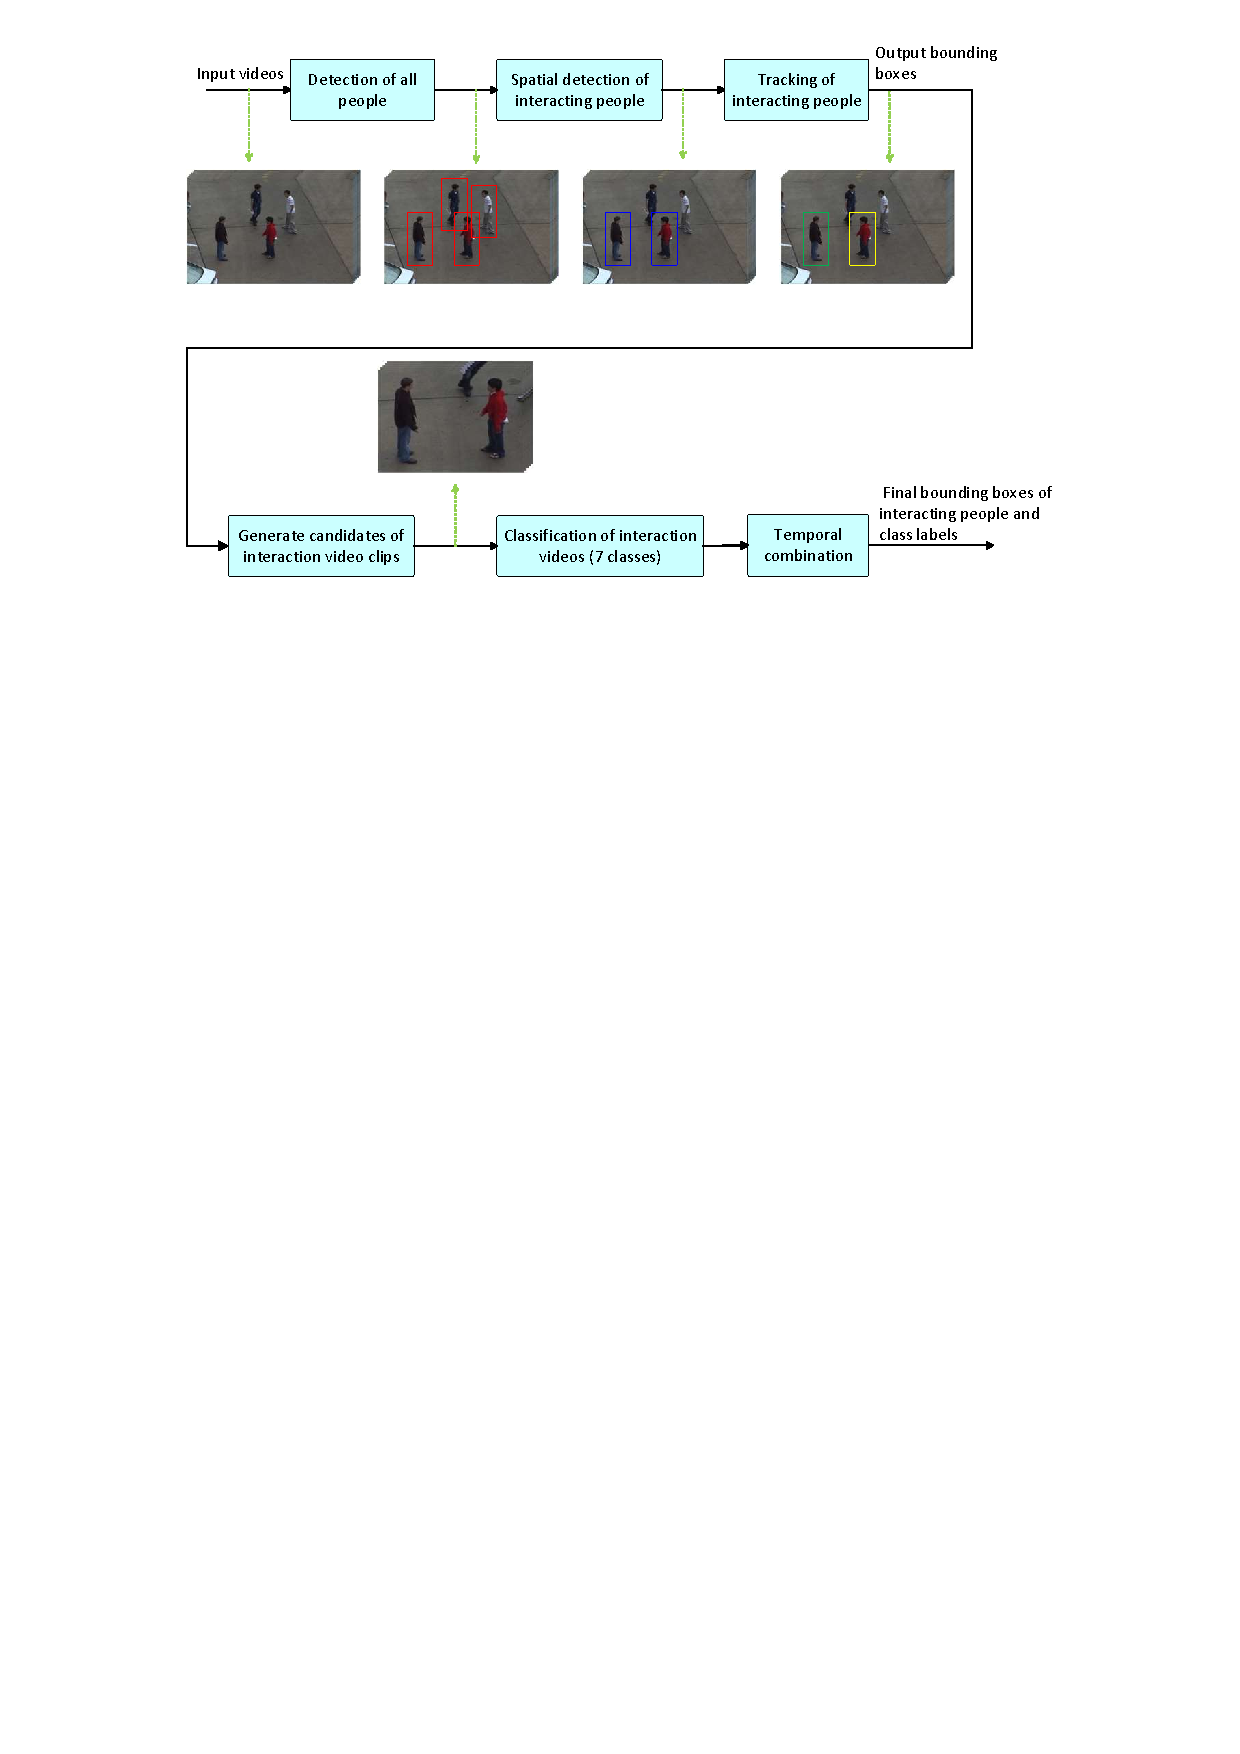
\includegraphics[trim=2cm 19.5cm 0cm 1cm]{fig01/interaction_detection.pdf}
	\caption{The data-flow of interaction detection}
	\label{fig:interaction_detection}
\end{figure}

\subsection{Detection of all people}
We use a person detector which is the same as that in the Section \ref{personDetection} to locate all people in each frame of the input videos. We input the unsegmented videos provided by UT-Interaction dataset for detection tasks to the person detector, and get the detected locations in each frame of each input video. An example illustration of the input and output of the person detection is shown in Figure \ref{fig:interaction_detection}.

\subsection{Spatial detection and tracking of interacting people}
\label{locate_interacting_people}
The output of the person detector are bounding boxes of all detected people of the input videos, those irrelevant people present in the videos will be selected out also as shown in the Figure \ref{fig:interaction_detection}.  So, the purpose of spatial detection of interacting people is to locate the interacting people and ignore those irrelevant people. We first introduce the main nations and basic assumptions which we apply to spatial detection and tracking of interacting people, followed by the detail methods. 

\subsubsection*{Notations and assumptions}
\paragraph*{Notations}
We define some notations for the bounding boxes of individual and two-person interaction as shown in Figure \ref{fig:bb_notations}. For the bounding box of an individual, we notate its left-top and right-bottom points  with \((x_A,y_A)\) and \((x_B,y_B)\) respectively, and:
\begin{eqnarray}
	width = x_B - x_A \\
	hight = y_B - y_A \\
	(x_{mid}, \quad y_{mid}) = (x_A + \frac{width}{2},\quad y_A + \frac{height}{2})
\end{eqnarray}
\begin{figure}
	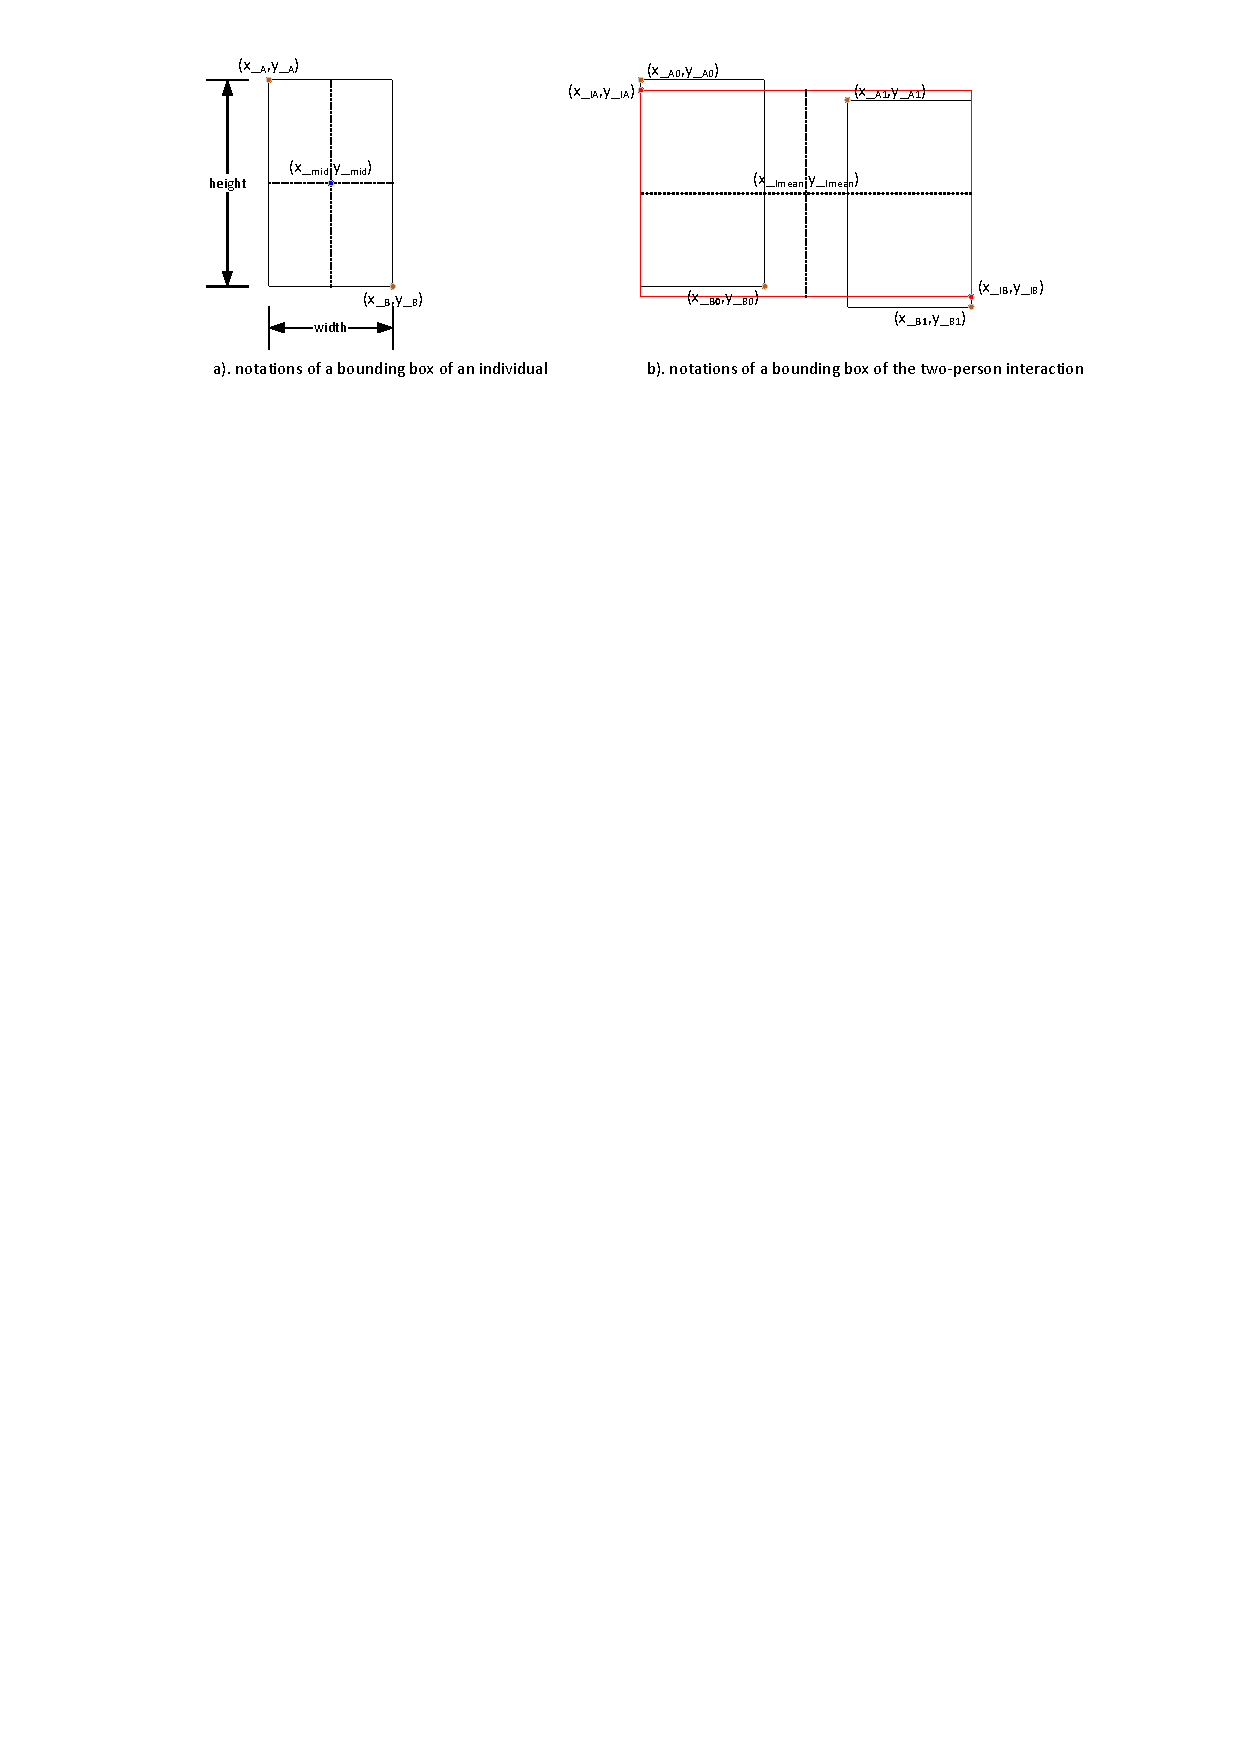
\includegraphics[trim=2cm 23cm 0cm 1cm]{fig01/bb_notations.pdf}
	\caption{Illustrations of notations of bounding boxes, a). notations of a bounding boxes of an individual and b). notations of a bounding box of two-person interaction.}
	\label{fig:bb_notations}
\end{figure}
And for the bounding box of the two-person interaction, we have definitions and notations as below:
\begin{eqnarray}
	(x_{IA}, \quad y_{IA})\,  = \ ({x_{A0}, \quad \frac{y_{A0} + y_{A1}}{2}}) \\
	({x_{IB}, \quad y_{IB}})\,  = \  ({x_{B1}, \quad \frac{y_{B0} + y_{B1}}{2}}) \\
	(x_{Imean}, y_{Imean}) \, = \, (\frac{x_{IA} + x_{IB}}{2}, \quad \frac{y_{IA} + y_{IB}}{2})
\end{eqnarray}
Where \(x_{Ai},y_{Ai},x_{Bi},y_{Bi}\) are the coordinates of the \(ith\) bounding box of the  individuals, \(x_{IA},y_{IA},x_{IB},y_{IB}\) are the coordinates of the bounding box of two-person interaction, and \(x_{Imean},y_{Imean}\) are the coordinates of the center point of the interaction bounding box.

\paragraph*{Assumptions}
To find out the interacting people from all people who present in the videos, we have following basic assumptions: 
\begin{enumerate}
	\item All individuals have similar size of bounding boxes. We design a method to learn a stable width and height of bounding box and apply them for all individuals. By doing this, those over-small or over-large bounding boxes caused by the mistakes of the person detection will be eliminated.
	\item The horizon positions of the interacting people are very close, which is illustrated in Figure \ref{fig:interacting_people}.
	\item The moving speed of an interaction bounding box is slow between two successive frames.
\end{enumerate}

\begin{figure}
	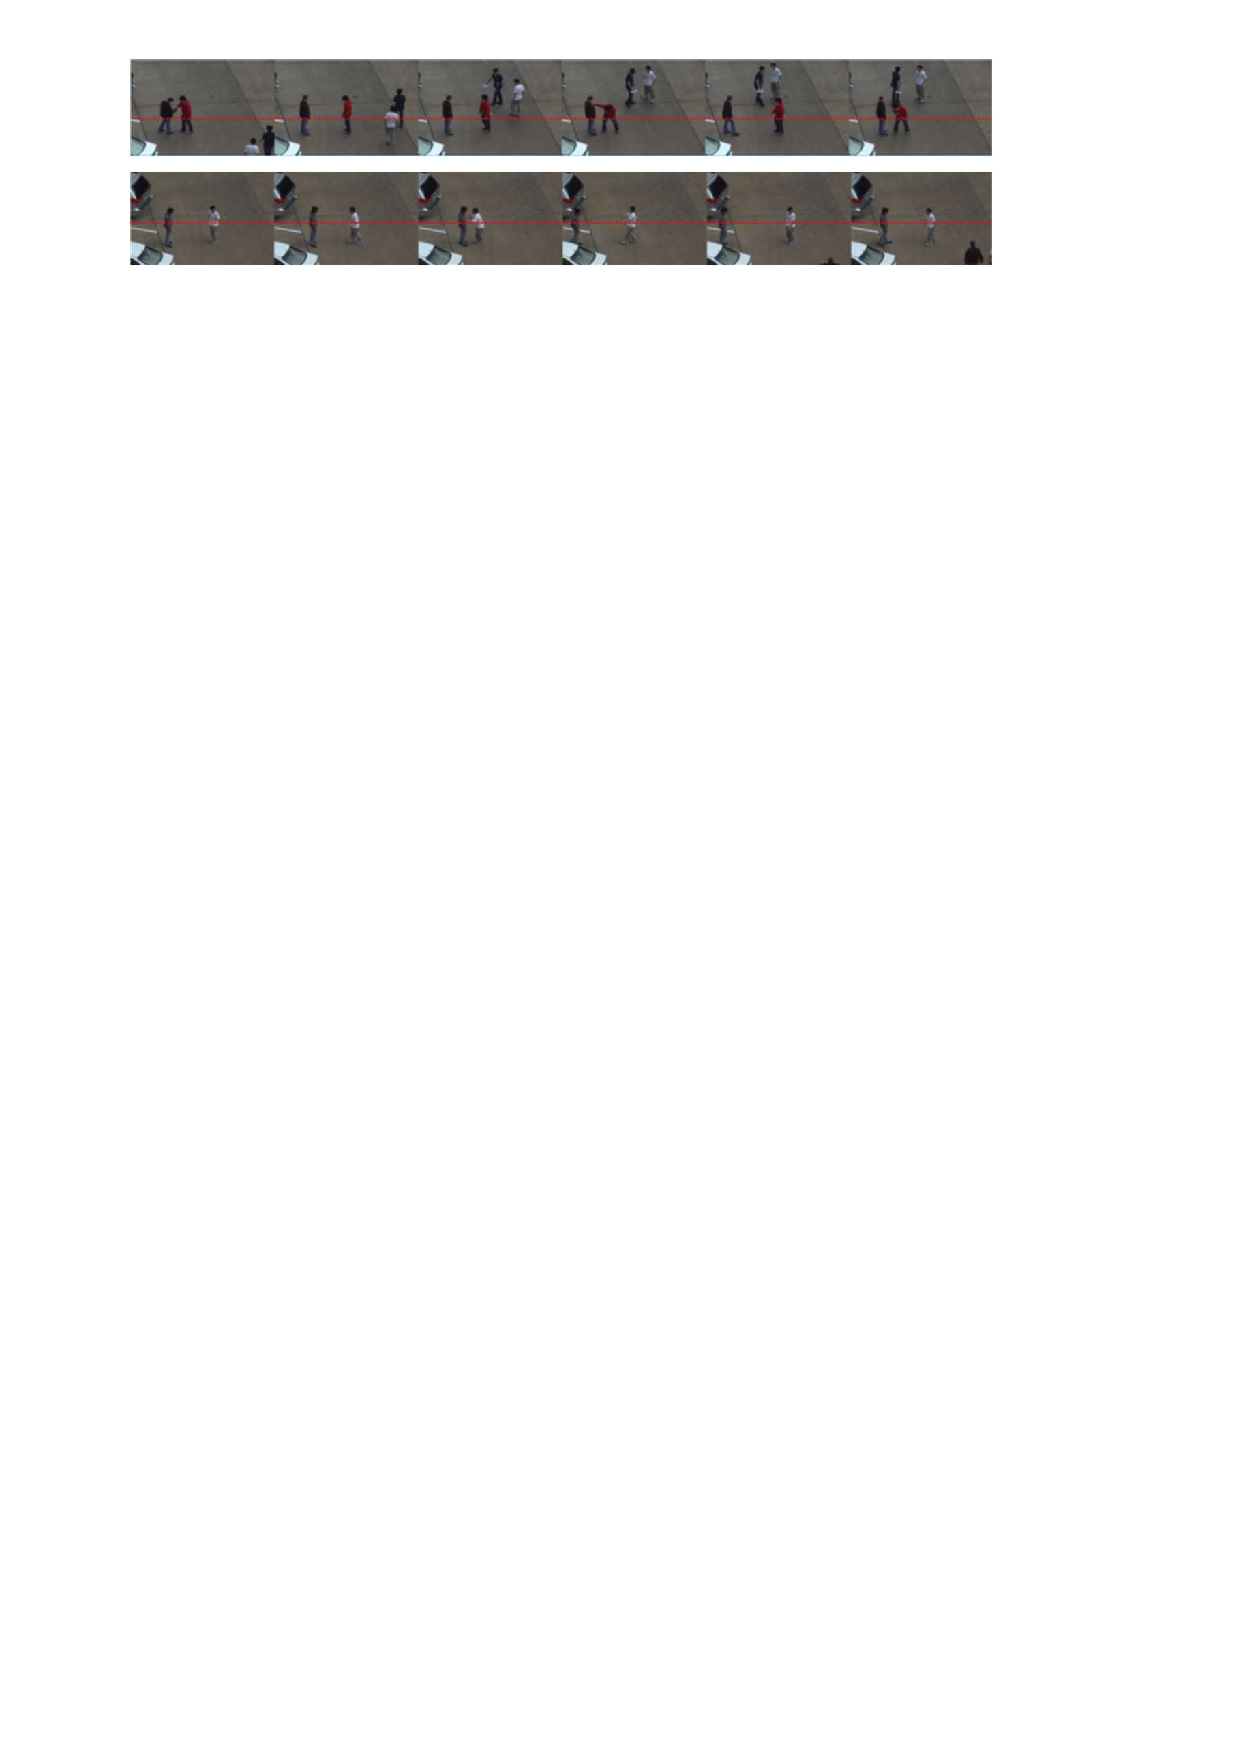
\includegraphics[trim=2cm 24.5cm 0cm 1cm]{fig01/interacting_people.pdf}
	\caption{Some examples of the horizon positions of the interacting people, sampled from the unsegmented videos of UT-Interaction dataset.}
	\label{fig:interacting_people}
\end{figure}

\subsubsection*{Learn the stable width and height of the bounding boxes for individuals}
We assume that the bounding boxes of all individuals have same width and height throughout a whole video. So, we design a method to learn such a width and height. We learn the value of width with the formulas as below and learn the value of height in the same way. 
\begin{eqnarray}
	w_1^t = Norm\left(\frac{1}{abs(width_i^{t-1} - width_i^t)}\right) \\
	w_2^t = Norm\left(\frac{1}{Min(abs(width_i^t - width_{\bar i}^t))}    \right) \\
	width_t = \sum_{i=0}^N width_i^t \times (0.5 \times w_{1i}^t + 0.5 \times w_{2i}^t)
\end{eqnarray}
Where \(w_{1}^t\) is the temporal learning weight which puts more weights on those new bounding boxes of which the value of width is closer to the learned width, \(w_{2}^t\) is the spatial learning weight which puts more weights to those new bounding boxes which has very similar width with each other in the same frame. \(Norm(X_i) = \frac{X_i}{\sum_i X_i} \) is a vector normalization function. \(width_i^t\) is the value of the width of the \(ith\) bounding box at time \(t\), and \(width_{\bar i}^t\) are the values of the width of the other bounding boxes except the \(ith\) one at time \(t\).  
\par 
By applying above method, the learned width and height can be more general represent the width and height of each individual's bounding box. And those bounding boxes with area less than \(0.75\times widht \times height \) or larger than \(1.25 \times width \times height\) are discarded as false positive detections. 

\subsubsection*{Learn the value of \(X_{Imean}\) and \(Y_{Imean}\)}
We have previously defined \(X_{Imean}\) and \(Y_{Imean}\) as the coordinates of the center point of the interaction bounding box. 	Since we do not previously know the positions of interacting people, then value of  \(X_{Imean}\) and \(Y_{Imean}\) can not be calculated directly. We learn the value of  \(X_{Imean}\) and \(Y_{Imean}\) from the bounding boxes of all people. 
\paragraph*{Learn the value of \(Y_{Imean}\)}
We assume that the interacting people usually stand in a very close horizontal position, thus we put more weights to those bounding boxes which have very close values of \(y_{mid}\). And we assume that the value of \(Y_{Imean}\) change very slowly, so, we put more weights to those  bounding boxes of which the values of \(y_{mid}\) are close to current \(Y_{Imean}\). We learn the value of \(Y_{Imean}\) with following formulas:
\begin{eqnarray}
	w_1^t = Norm\left(\frac{1}{|Y_{Imean}^{t-1} - y_{mid\_i}^t|}\right) \\
	w_2^t = Norm\left(\frac{1}{Min(|y_{mid\_i}^t - y_{mid \_ \bar i}^t|)}    \right) \\
	Y_{Imean}^t = \sum_{i=0}^N y_{mid\_i}^t \times (0.5 \times w_{1i}^t + 0.5 \times w_{2i}^t)
\end{eqnarray}

To further stably learn the value of \(Y_{Imean}\), we add an additional parameter \(learning\_rate\) to slow the learning rate of \(Y_{Imean}\) if its value is stable. We detect the stability of the values of \(Y_{Imean}\) and calculate \(learning\_rate\) with the following formulas: 
\begin{eqnarray}
	Y_{Imean}\_List = [Y_{Imean}^t,Y_{Imean}^{t-1},...,,Y_{Imean}^{t-19}] \\
	\mu = \frac{1}{20}\sum_{i=0}^{19}Y_{Imean}\_List_i \\
	std = \sqrt{\frac{1}{20}\sum_{i=0}^{19}(Y_{Imean}\_List_i - \mu)^2} \\
	learning\_rate = Min(1,std/20) \\
	Y_{Imean}^t \leftarrow Y_{Imean}^{t-1} + learning\_rate \times (Y_{Imean}^{t} - Y_{Imean}^{t-1})
\end{eqnarray}
Where \(Y_{Imean}\_List\) is a vector which contains 20 history values of \(Y_{Imean}\), \(\mu\) and \(std\) are the mean value and standard deviation of the list \(Y_{Imean}\_List\).
We only preserve those bounding boxes of which the distances between \(Y_{Imean}\) and \(y_{mid}\) are less than a small value \(thld\_y\). An example illustration of preserving and discarding bounding boxes according to the value of \(Y_{Imean}\) is shown in Figure \ref{fig:y_mean}.
\begin{figure}
	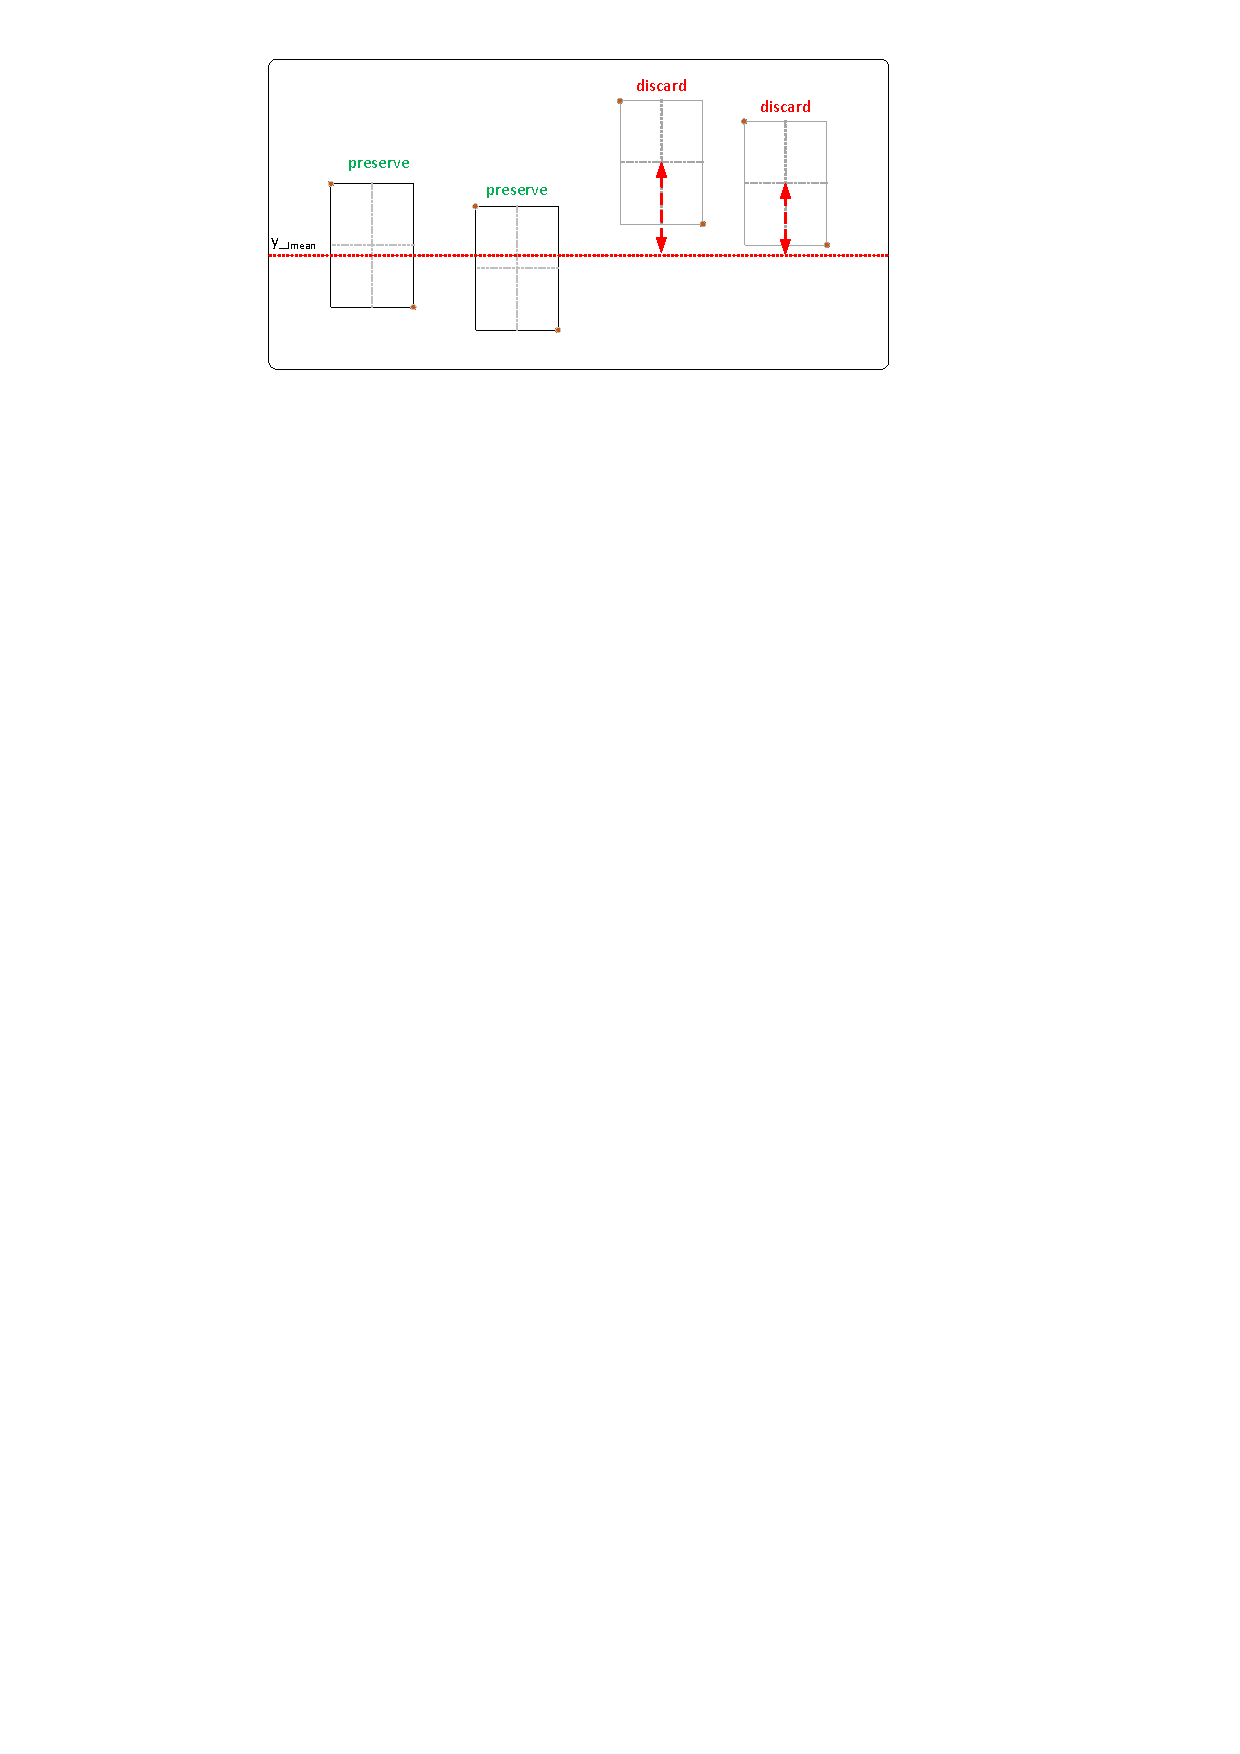
\includegraphics[trim=2cm 23cm 0cm 1cm]{fig01/y_mean.pdf}
	\caption{An example illustration of preserving and discarding bounding boxes according to the value of \(Y_{Imean}\)}
	\label{fig:y_mean}
\end{figure}
\paragraph*{Learn the value of \(X_{Imean}\)}
We learn the value of \(X_{Imean}\) from the preserved bounding boxes in the previous step with following formulas: 
\begin{eqnarray}
 	X_{mean} = \sum_{i=1}^M x_{mid\_i} \\
 	learning\_rate1 = \frac{1}{Max(1,\sqrt{|X_{Imean} - X_{mean}|}} \\
 	X_{Imean}\_List = [X_{Imean}^t,X_{Imean}^{t-1},...,,X_{Imean}^{t-19}] \\
 	\mu = \frac{1}{20}\sum_{i=0}^{19}X_{Imean}\_List_i \\
 	std = \sqrt{\frac{1}{20}\sum_{i=0}^{19}(X_{Imean}\_List_i - \mu)^2} \\
 	learning\_rate2 = Min(1,std/20) \\
 	X_{Imean}^t = X_{Imean}^{t-1} + learning\_rate1 \times learning\_rate2 \times (X_{mean}^{t} - X_{Imean}^{t-1})
\end{eqnarray}
Where \(X_{mean}\) is the mean value of \(x_{mid}\) of the preserved bounding boxes in the previous step. \(learning\_rate1\) is determined by the distance between the \(X_{mean}\) and current \(X_{Imean}\) and \(learning\_rate2\) is determined by the stability of history values of  \(X_{Imean}\). By doing this, we update the value of \(X_{Imean}\) slowly if the new \(X_{mean}\) is far away from \(X_{Imean}\) or the value of \(X_{Imean}\) is already get stable.
We then use the value of \(X_{Imean}\) to discard those bounding boxes which are far away from the vertical axis defined by the value of \(X_{Imean}\) and only preserve one bounding boxes in each side of the vertical axis. Some examples illustrate how we preserve and discard bounding boxes according to the value of \(X_{Imean}\) are shown in Figure \ref{fig:x_mean}.
\begin{figure}
	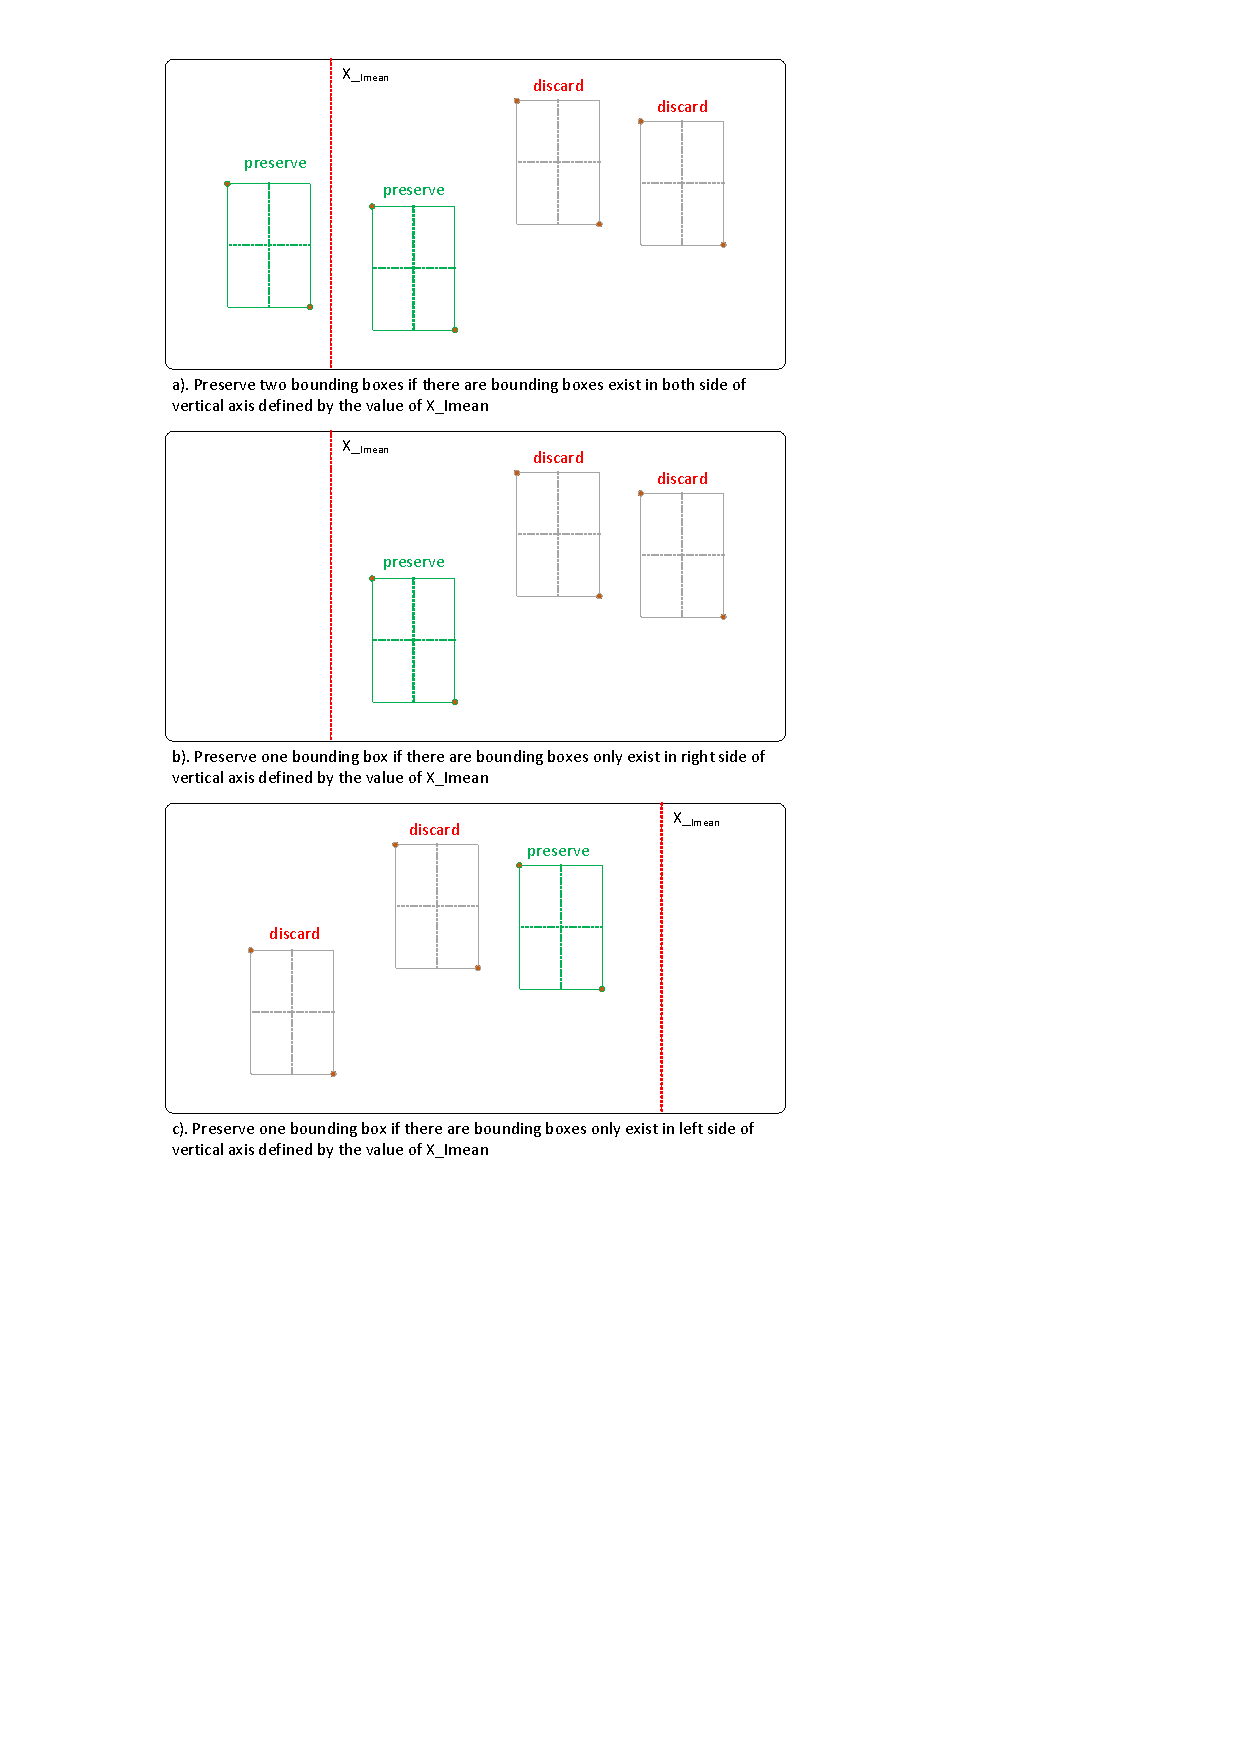
\includegraphics[trim=2cm 10cm 0cm 1cm]{fig01/x_mean.pdf}
	\caption{An example illustration of preserving and discarding bounding boxes according to the value of \(X_{Imean}\)}
	\label{fig:x_mean}
\end{figure}

\subsubsection*{Tracking of interacting people}
After discarding those bounding boxes according to the learned values of width, height, \(Y_{Imean}\) and \(X_{Imean}\), we get the bounding boxes of interacting people. Since detections may loss in some frames, we use the Kalman filters to track the locations for each person involved in the interaction. 

\subsection{Generate candidates of interaction video clips}
We generate the candidates of interaction videos clips by temporally sliding a 3D window with a fixed length \(l\) and temporal stride \(s\).  The illustration of sliding the 3D windows which are used to generate candidates of interaction video clips is shown in Figure \ref{fig:sliding_window}. And the coordinates of the sliding windows are calculated with following formulas:
\begin{eqnarray}
	(x_{IA\_i},y_{IA\_i}) = (\frac{\sum_{j=i*s}^{i*s+l} x_{A\_j}}{l}, \quad \frac{\sum_{j=i*s}^{i*s+l} y_{A\_j}}{l})   \quad \quad i \in \{0,1,2,...\} \\
	(x_{IB\_i},y_{IB\_i}) = (\frac{\sum_{j=i*s}^{i*s+l} x_{B\_j}}{l}, \quad \frac{\sum_{j=i*s}^{i*s+l} y_{B\_j}}{l})   \quad \quad i \in \{0,1,2,...\}	
\end{eqnarray}
Where \(x_{A\_j}, y_{A\_j}, x_{B\_j}, y_{B\_j}\) are the coordinates of the spatial bounding box of interacting people in the \(jth\) frame. 
\begin{figure}
	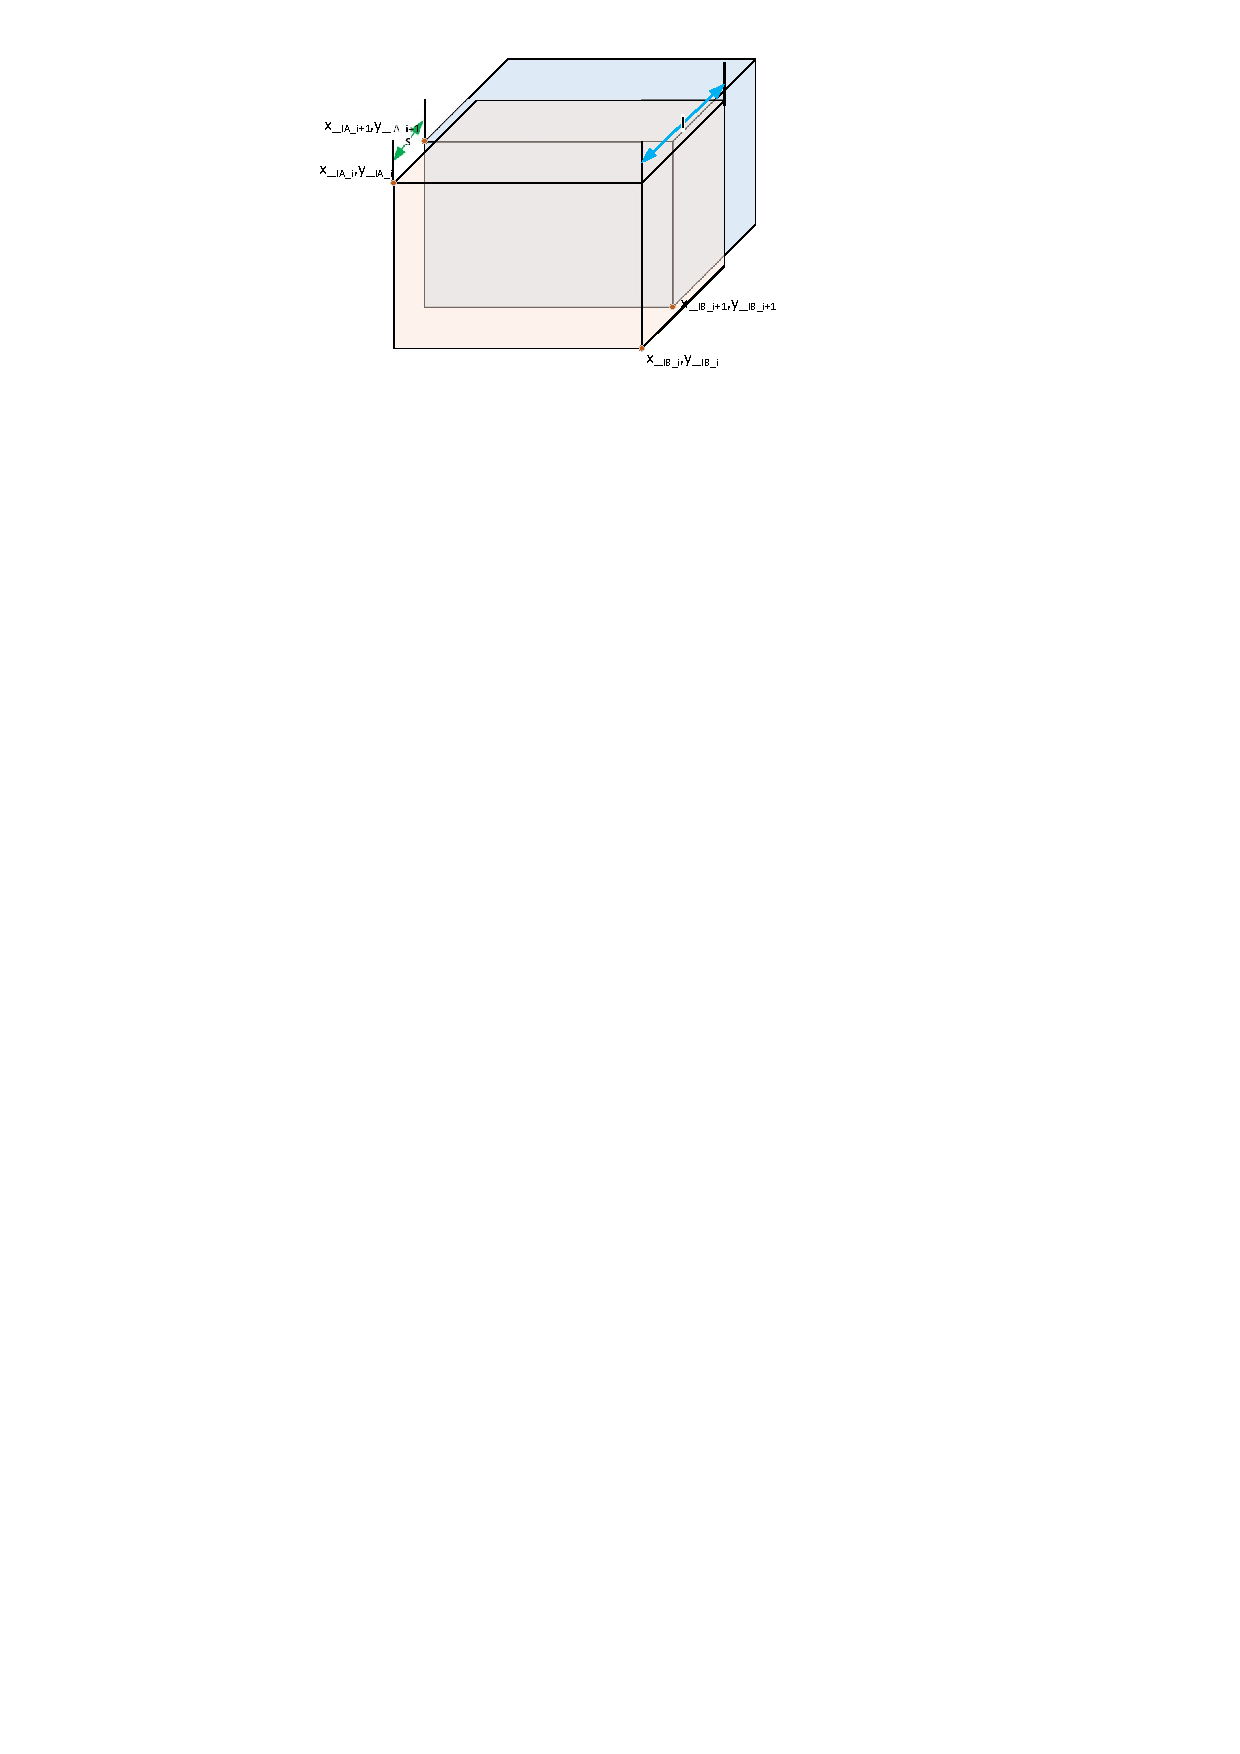
\includegraphics[trim=2cm 23.5cm 0cm 1cm]{fig01/sliding_window.pdf}
	\caption{The illustration of temporally sliding the 3D windows which are used to generate candidates of interaction video clips.}
	\label{fig:sliding_window}
\end{figure}

\subsection{Classification of interaction video clips}
The interaction classifier we trained in the classification task has only 6 classes, but in the detection task, we need an additional class to label those video clips which do not belong to one of the 6 positive classes. 
\subsubsection*{Training of interaction classifier for detection task}
\label{extra_class}
The UT-Interaction dataset only provides training videos for the 6 positive classes, so we generate a batch of video clips by randomly cropping in the unsegmented videos, and for each that does not overlap with any positive bounding boxes. We keep those new boxes as negative training video clips. For simplicity, we use the average width and height of all positive bounding boxes as the values of the width and height of the negatives and the number of frames for each negative video clip is fixed to 64.  We then use all the positive and negative training video clips to train our interaction classifier (7 classes). 
\par 
We apply the trained interaction classifier (7 classes) to predict the class labels for all candidates of interaction video clips and get the results in the format as below for each candidate: \(\{Start\_No., End\_No., x_A,y_A,x_B,y_B,class\_lable\}\).  
 
\subsection{Temporal combination} 
We first drop those candidates with negative predicted class\_labels, then temporally combine those candidates which have successive \(Start\_No\) as shown in Figure \ref{fig:temporal_combination}.
\begin{figure}
	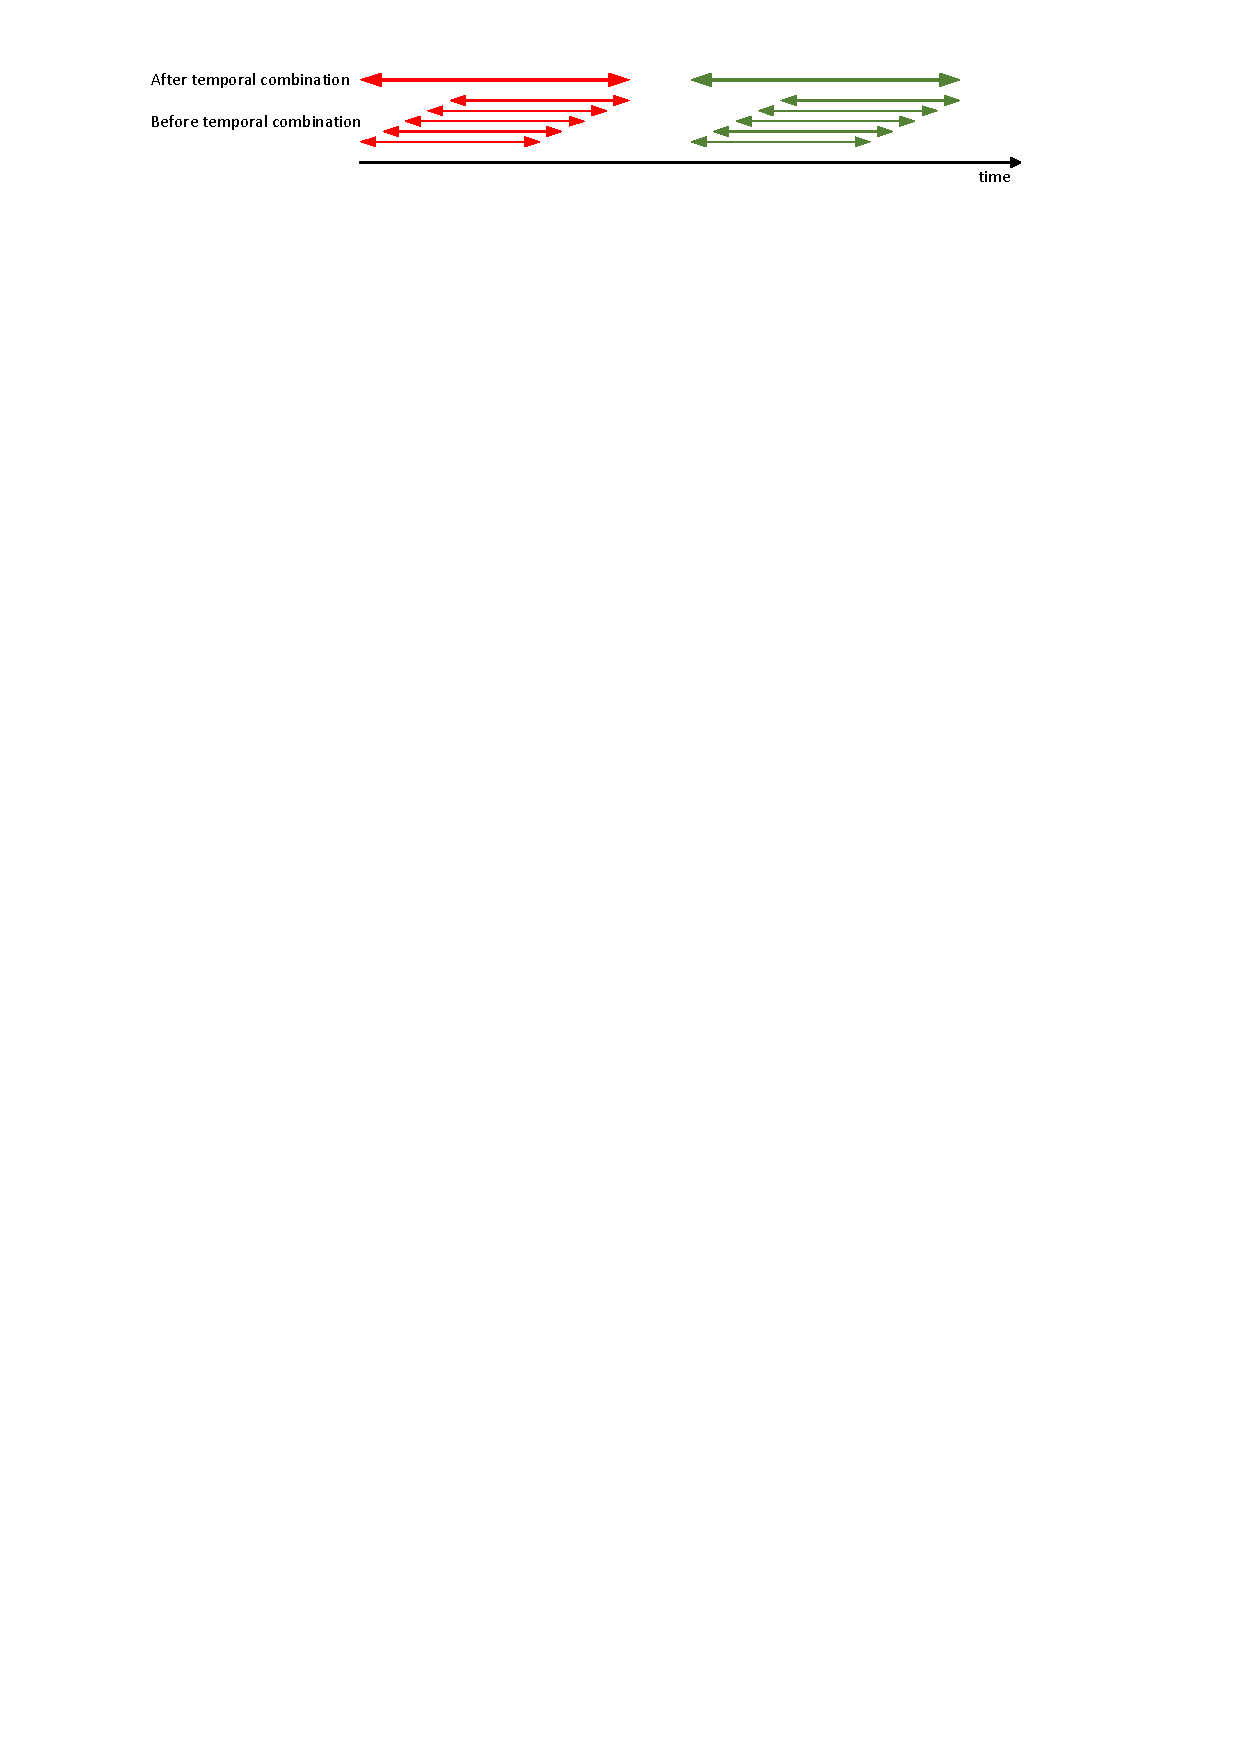
\includegraphics[trim=2cm 27cm 0cm 1cm]{fig01/temporal_combination.pdf}
	\caption{A diagram of temporally combining of interaction video clips }
	\label{fig:temporal_combination}
\end{figure}

After temporal combination of candidates, we get many combined candidates which consist of server original candidates in each. Since the predicted class labels of original candidates in a single combination may be different, we use the majority rule to vote a class label as the final class label for the combination. For example, a combined candidate consist of 5 original candidates which have predicted class labels \([2,3,3,3,1]\), then we take \(3\) as its final class label.
%=========================================================